\documentclass[10pt,a4paper,twoside]{report}
\usepackage[utf8]{inputenc}

\usepackage[]{feupteses}
%\usepackage[square,sort,comma,numbers]{natbib}


\usepackage[english]{babel}




%\bibliographystyle{IEEEtran}

%\usepackage[square]{natbib}
\usepackage{graphicx}
\usepackage{framed}
\usepackage{multirow}
\usepackage{lipsum}  
\usepackage{verbatim}
\usepackage{amsmath}
\usepackage{longtable}
\usepackage{caption}
\usepackage{subcaption}
\usepackage{varwidth}

\usepackage{array}
\usepackage{adjustbox}

\usepackage{booktabs}


%\usepackage[oneside,width=17.5cm,height=24cm,left=2cm]{geometry}
%\usepackage[nolist,nohyperlinks]{acronym}

\usepackage[]{nomencl}
\usepackage[final]{pdfpages}

%\usepackage{biblatex}
%\addbibresource{references.bib}
\usepackage{mdframed}


\newcolumntype{L}[1]{>{\raggedright\let\newline\\\arraybackslash\hspace{0pt}}m{#1}}
\newcolumntype{C}[1]{>{\centering\let\newline\\\arraybackslash\hspace{0pt}}m{#1}}
\newcolumntype{R}[1]{>{\raggedleft\let\newline\\\arraybackslash\hspace{0pt}}m{#1}}

%%%  para ter capítulos xpto
%%%  https://hstuart.dk/2007/05/21/styling-the-chapter/


\usepackage{tikz, blindtext}
\usepackage{kpfonts}
\usepackage[explicit]{titlesec}
\usepackage{xcolor}
\definecolor{FEUP_color}{RGB}{140,45,25}

\newcommand*\chapterlabel{}
\titleformat{\chapter}
{\gdef\chapterlabel{}
	\normalfont\sffamily\huge\bfseries\scshape}
{\gdef\chapterlabel{\thechapter\ }}{0pt}
{\begin{tikzpicture}[remember picture,overlay]
	\node[yshift=-6cm] at (current page.north west)
	{\begin{tikzpicture}[remember picture, overlay]
		%\draw[fill=white] (-1,0) rectangle
	%	(1.2\paperwidth,8cm);
		\node[anchor=west,xshift=3cm,rectangle,
		rounded corners=1pt,inner sep=11pt,
		fill=black]
		{\color{white}\chapterlabel#1};
		\end{tikzpicture}
	};
\end{tikzpicture}
}
\titlespacing*{\chapter}{0pt}{50pt}{50pt}

\makenomenclature
\chapter*{Acronyms}
%\addcontentsline{toc}{chapter}{Acronyms}

%----------------------
%Acronyms List 
%----------------------
{
	\footnotesize
\begin{flushleft}
	\begin{tabular}{l p{0.8\linewidth}}
		
		\\
		
		AC	&	Alternating Current	\\
		AMR	&	Automatic Meter-Reading system	\\
		CEBD	&	Compiled Energy Billing Data-sets	\\
		DC	&	Direct Current	\\
		DCS	&	Data Collecting System	\\
		DHS	&	Data Handling System	\\
		DSS	&	Decision Support System	\\
		DSSS	&	Direct Sequence Spread Spectrum	\\
		FEM	&	Finit Element Method	\\
		EMI	&	Electromagnetic Interference	\\
		EETC	&	Energy-efficient Train Control	\\
		EETT	&	Energy-Efficient Train Timetabling	\\
		EMF	&	Energy Measurement Function	\\
		EMS	&	Energy Measurement System	\\
		ERA	&	European Union Agency for Railways	\\
		EU	&	European Union	\\
		GMSK	&	Gaussian Minimum Shift Keying	\\
		GPS	&	Global Position System	\\
		GSM	&	Global System for Mobile communications	\\
		GTO	&	Gate Turn-off Thyristors	\\
		ICT	&	Information and Communication Technology	\\
		IGBT	&	Insulated Gate Bipolar Transistors	\\
		IP	&	Internet Protocol	\\
		IP3	&	Innovation Programme 3	\\
		ISM	&	Industrial, Scientific and Medical	\\
		KPI	&	Key Performance Indicators	\\
		LAN	&	Local Area Network	\\
		LC	&	Inductor-Capacitor	\\
		LTE	&	Long-Term Evolution	\\
		MAC	&	Medium Access Control	\\
		MDMS	&	Meter Data Management System	\\
		OFDM	&	Orthogonal Frequency Division Multiplexing	\\
		OSI	&	Open Systems Interconnection	\\
		PLC	&	Power Line Communication	\\
		QoS	&	Quality of Service	\\
		PHY	&	Physical Layer	\\
		RTS	&	Railway Transportation System	\\
		RUs	&	Railway Undertakings	\\
		S2R	&	Shift2Rail	\\
		SG	&	Smart Grid	\\
		SMD	&	Smart Metering Demonstrator	\\
		TCMS	&	Train Communication \& Management System	\\
		TSIs	&	Technical Specifications for Interoperability	\\
		WLAN	&	Wireless LAN	\\
		WSN	&	Wireless Sensor Networks	\\

		
		
		
		
	\end{tabular}
\end{flushleft}
}
%----------------------
% Automatic Acronyms Generator
%----------------------
\acrodef{}{}

\acrodef{AC}{Alternating Current}
\acrodef{AMR}{Automatic Meter-Reading system}
\acrodef{CEBD}{Compiled Energy Billing Data-sets}
\acrodef{DC}{Direct Current}
\acrodef{DCS}{Data Collecting System}
\acrodef{DHS}{Data Handling System}
\acrodef{DSS}{Decision Support System}
\acrodef{DSSS}{Direct Sequence Spread Spectrum}

\acrodef{FEM}{Finit Element Method}
\acrodef{EMI}{Electromagnetic Interference}
\acrodef{EETC}{Energy-efficient Train Control}
\acrodef{EETT}{Energy-Efficient Train Timetabling}
\acrodef{EMF}{Energy Measurement Function}
\acrodef{EMS}{Energy Measurement System}
\acrodef{ERA}{European Union Agency for Railways}
\acrodef{EU}{European Union}
\acrodef{GMSK}{Gaussian Minimum Shift Keying}
\acrodef{GPS}{Global Position System}
\acrodef{GSM}{Global System for Mobile communications}
\acrodef{GTO}{Gate Turn-off Thyristors}
\acrodef{ICT}{Information and Communication Technology}
\acrodef{IGBT}{Insulated Gate Bipolar Transistors}
\acrodef{IP}{Internet Protocol}
\acrodef{IP3}{Innovation Programme 3}
\acrodef{ISM}{Industrial, Scientific and Medical}

\acrodef{KPI}{Key Performance Indicators}
\acrodef{LAN}{Local Area Network}
%\acrodef{LC}{Inductor-Capacitor}
\acrodef{LTE}{Long-Term Evolution}
\acrodef{MAC}{Medium Access Control}
\acrodef{MDMS}{Meter Data Management System}
\acrodef{OFDM}{Orthogonal Frequency Division Multiplexing}
\acrodef{OSI}{Open Systems Interconnection}
\acrodef{PLC}{Power Line Communication}
\acrodef{QoS}{Quality of Service}
\acrodef{PHY}{Physical Layer}

\acrodef{}{}
\acrodef{RTS}{Railway Transportation System}
\acrodef{RUs}{Railway Undertakings}
\acrodef{S2R}{Shift2Rail}
\acrodef{SG}{Smart Grid}
\acrodef{SMD}{Smart Metering Demonstrator}
\acrodef{TCMS}{Train Communication \& Management System}
\acrodef{TSIs}{Technical Specifications for Interoperability}
\acrodef{WLAN}{Wireless LAN}
\acrodef{WSN}{Wireless Sensor Networks}



\renewcommand{\bibname}{References}%





%some macro definitions

% format
\newcommand{\class}[1]{{\normalfont\slshape #1\/}}

% entities
\newcommand{\Feup}{Faculdade de Engenharia da Universidade do Porto}

\newcommand{\svg}{\class{SVG}}
\newcommand{\scada}{\class{SCADA}}
\newcommand{\scadadms}{\class{SCADA/DMS}}


\begin{document}

%%----------------------------------------
%% Information about the work
%%----------------------------------------
\title{Smart Metering towards energy efficiency increasing in railways systems}

\author{Vítor A. Morais}

%% Uncomment next line if necessary for degree
\degree{Programa Doutoral em Engenharia Electrotécnica e de Computadores}

%% Uncomment next line for date of submission
%\thesisdate{July 31, 2016}

%% Uncomment next line for copyright text
%\copyrightnotice{Name of the Author, 2016}

\supervisor{Supervisor}{António P. Martins}

%% Uncomment next line if necessary
%\supervisor{Second Supervisor}{Name of the Supervisor}

%% Uncomment committee stuff in the final version if used
%\committeetext{Approved by \ldots:}
%\committeemember{President}{Name of the President}
%\committeemember{Referee}{Name of the Referee}
%\committeemember{Referee}{Name of the Referee}

%% Uncomment signature line in the final on paper version if used
%\signature

%% Specify cover logo (in folder ``figures'')
\logo{figures/uporto.pdf}

%% Uncomment next line for additional text below the author's name (front page)
\additionalfronttext{DRAFT VERSION}



%\chapter*{Abstract}
%Abstract goes here
%%
%%   Section 
%%
\begin{Prolog}
\cleardoublepage

\tableofcontents


%\printnomenclature

%\chapter*{Symbols}
%\begin{flushleft}

\begin{tabular}{l p{0.8\linewidth}}


kbps     & Kilobit per second (often used kbit/s or kb/s) - bit rate\\
Mbps     & Megabit per second (often used Mbit/s or Mb/s) - bit rate\\
Gbps     & Gigabit per second (often used Gbit/s or Gb/s) - bit rate\\
dB       & Decibel - Gain/Attenuation\\
kHz      & Kilohertz - Frequency\\
MHz      & Megahertz - Frequency\\
GHz      & Gigahertz - Frequency\\
km       & Kilometer - Distance\\
min      & Minute - Time\\


\end{tabular}
\end{flushleft}

	
\end{Prolog}

\StartBody

\chapter{Introduction}
\lipsum[4-4]


\chapter{Objectives and Contributions}





\section{Objectives}

This work is focused on measuring the energy flows in the railway system.
The aim of this work is to improve the energy efficiency in the railway transportation system (RTS) and reduce the maintenance cost of RTS power systems.
The implementation of smart meters (SM) in RTS promote a better overview of power flow and, based on the information of SM, algorithms focusing on energy efficiency can be implemented.
The SM requires sensors such as voltage and current sensors. The level of intrusion as well as the level of electric <<valor da grandeza electrica>> of such sensors implies considerable costs of the sensors.
Therefore, the implementation of complex processing on smart meters is of added value. This complex processing can be the implementation of fault monitoring algorithms in SM based on the energy measurements.
Framed in the shif2rail, the work is focused on the implementation of a smart meter demonstrator for the RTS. To embrace the entire railway system, the power flow should consider the energy flux from and to the catenary. Therefore, the key point should be the measurement of the energy in the traction substations and in the train power transformer 
Based on this thesis proposal, the objectives are the following:

\begin{itemize}
	\setlength\itemsep{0em}
	
	\item	Modeling, development and implementation of a metering system based on a non-intrusive self-powered sensor node.

	\item Modeling and simulation of a RTS wireless network.

	
\end{itemize}


\section{Contributions}

\begin{itemize}
	\setlength\itemsep{0em}
	
	\item Availability of measured data from trains where currently no energy measurement is performed.
	
	\item Data-rate increase of energy measurements, which will result on direct increase on the quality of information of energy.
	
	\item A further contribution can be the avoidance of broadband real-time/continuous communication (such as LTE), being possible to collect and store data in train data concentrator and, while the train is waiting at stations, the data is transferred between train and station AP (and then to a remote server). A possible contribution will be the cost reduction of information transmission of energy sensor network data.
	
	\item New advanced sensor node for AC current measurement;
	
	\item Possible contribution: Given the measurement characteristics, a self powered wireless sensor node can implement features of high processing.
	
\end{itemize}







\chapter{Literature Review}
%\lipsum[4-4]





%\section{Synthesis}

%\lipsum[4-4]



















\section{Section 1: Power system of RTS}


In this section is started the literature review of this document, with the coverage of the Railway Transportation System (RTS). This system is reported to transport <<need data>> of people and <<data>> goods. With high influence in the transportation of goods and people in the last century, this system had substantial technological enhancements. Currently we have a RTS with substantial differences in the supply system.

In subsection \ref{subs:311} is presented an overview on European railway electrical supply systems. Later on, in subsection \ref{subs:312}, a comparison between different catenary supply systems is presented and in subsection \ref{subs:313} is presented a comparison of the power system architecture of trains. A further detail on train electrical components is presented in subsection \ref{subs:314}.

This section is supported on the chapter 5 of the work of \cite{abad2016}. Further reading of this book chapter is advisable. 

\subsection{Overview of Existing European Railway Power Systems}
\label{subs:311}
Back to the 19th century, the steam turbine was the main propulsion system for the trains. Later on, electric and diesel propulsion systems were adopted. In recent years occurred a massive introduction of IGBT-based power converters, which allowed an increase of energy efficiency (allowing, for example, regenerative breaking and reduction of power losses in traction motors).

Due to this evolution, different topologies of the railway system exists nowadays. In table \ref{tab:31.t1}, different catenary topologies are visible which results in different power systems for RTS.


% Table generated by Excel2LaTeX from sheet 'Sheet1'
\begin{table}[htbp]
	\centering
	\tiny
	\caption{Catenary topology and vehicle characteristics of different railway vehicles. \cite{abad2016}.}
	\begin{tabular}{|c|p{10.145em}p{10.355em}|cc|}
		\cmidrule{2-5}    \multicolumn{1}{c|}{} & \multicolumn{2}{c|}{\textbf{Catenary topology}} & \multicolumn{2}{c|}{\textbf{Vehicle characteristics}} \\
		\cmidrule{2-5}    \multicolumn{1}{c|}{} & \multicolumn{1}{c}{\textbf{DC supply}} & \multicolumn{1}{c|}{\textbf{AC supply}} & \textbf{Power} & \textbf{Top speed} \\
		\midrule
		\textbf{Tram} & 600V DC, 750V DC, 900V DC & \multicolumn{1}{c|}{-}     & 150–300kW & 50–70km/h \\
		\midrule
		\textbf{Metro} & 750V DC, 1500V DC & \multicolumn{1}{c|}{-}     & 350kW–1MW & 80km/h \\
		\midrule
		\textbf{Train} & 750V DC, 1500V DC, 3000V DC & 15kV AC (16.7Hz) and 25kV AC (50Hz) & 200kW–8MW & 120–350km/h \\
		\midrule
		\textbf{Locomotive} & 750V DC, 1500V DC, 3000V DC & 15kV AC (16.7Hz) and 25kV AC (50Hz) & 500kW–8MW & 100–200km/h \\
		\bottomrule
	\end{tabular}%
	\label{tab:31.t1}%
\end{table}%


Across the Europe, RTS depends on different types of electrification systems, as it is illustrated in figure \ref{fig:abad2016}.


\begin{figure}[h!]
	\centering
	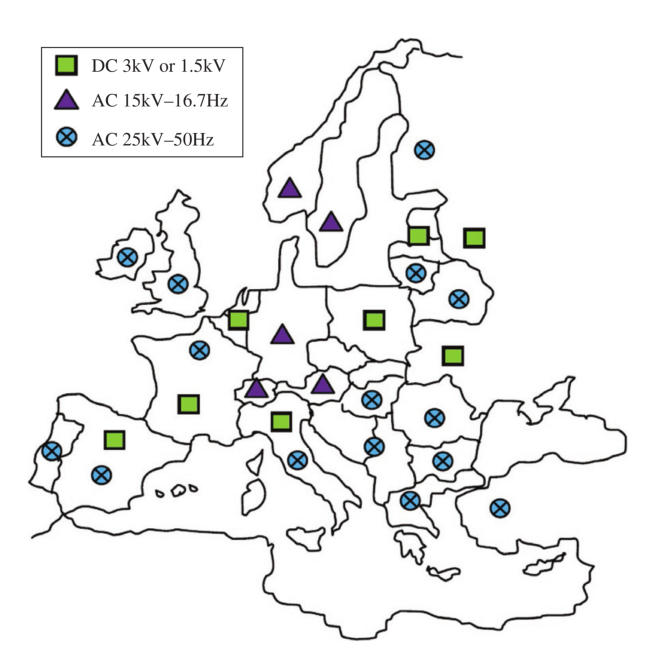
\includegraphics[width=0.7\textwidth,keepaspectratio]{figures/31.PowerS/abad2016}
	\caption{Railway main-line power supply systems in Europe. Adapted from \cite{abad2016}.}
	\label{fig:abad2016}
\end{figure}



\subsection{Railway Power Supply System}
\label{subs:312}

Similarly to the electrical grid where a broad area of loads must be supplied, the railway power system must be capable of maintaining trains running in a broad area. The energy is supplied to the railway system through traction substations, similarly to the generation units of the electrical grid.

These traction substations ensure the interface between the electrical grid and the railway system, being responsible of supplying the distribution line of the railway system - or catenary.

As previously referred, the catenary can be divided in three main topologies:

%\begin{itemize}
%	\setlength\itemsep{-0.5em}
%	
%	\item DC supply system (six-, or 12-pulse diode rectifiers);
%	
%	\item AC 50Hz (or 60Hz) supply system;
%	
%	\item AC 16.7Hz supply system;
%
%\end{itemize}

\paragraph{1. DC supply system\\}

The DC supply system depends on rectifier converters (controlled or uncontrolled) as illustrated in figure \ref{fig:abad2016b}. This railway power supply topology requires several traction substations, towards the reduction of power losses in catenary due to the high value of current. In figure \ref{fig:abad2016f} is presented the supply architecture of such lines.


\begin{figure}[h!]
	\centering
	\begin{minipage}{.5\textwidth}
		\centering
		%		\vspace{2.5em}
		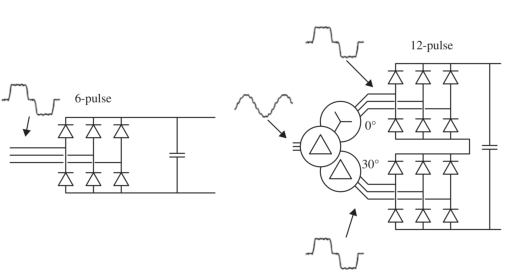
\includegraphics[width=\textwidth,keepaspectratio]{figures/31.PowerS/abad2016b}
		%		\vspace{2em}
		\captionof{figure}{6-pulse and 12-pulse diode rectifier configurations. Adapted from \cite{abad2016}.}
		\label{fig:abad2016b}
	\end{minipage}%
	\begin{minipage}{.03\textwidth}  ~\end{minipage}	
	\begin{minipage}{.4\textwidth}
		\centering
		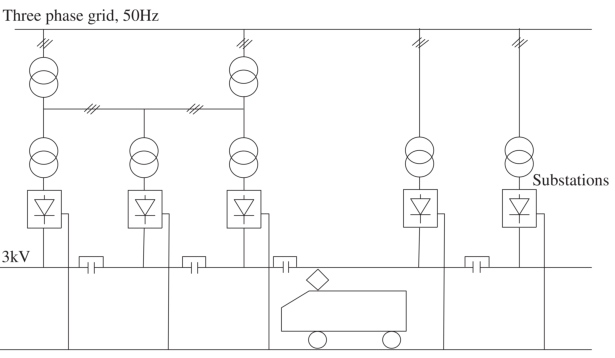
\includegraphics[width=\textwidth,keepaspectratio]{figures/31.PowerS/abad2016f}
		%		\vspace{0.5em}
		\captionof{figure}{DC supply system architecture. Adapted from \cite{abad2016}.}
		\label{fig:abad2016f}
	\end{minipage}
\end{figure}

\paragraph{2. AC 50Hz (or 60Hz) supply system\\}

With AC catenaries, low frequency single-phase transformer is required to step down the catenary voltage (25 kV or 15 kV) to the rectifier operating voltage (the rectifier is a single-phase voltage source converter, usually with bi-directional power flow).

On the traction substation, a special setup of power transformers avoids the usage of complete power converters. In figure \ref{fig:abad2016d} is presented the substation setup to supply a single-phase 50Hz catenary.

\paragraph{3. AC 16.7Hz supply systems\\}
An alternative setup is presented in figure \ref{fig:abad2016e} where a single-phase 16.7Hz supply voltage is generated with a complete power converter. 
%\vspace{-2.5em}


\begin{figure}[h!]
	\centering
	\begin{minipage}{.45\textwidth}
		\centering
		%		\vspace{2.5em}
		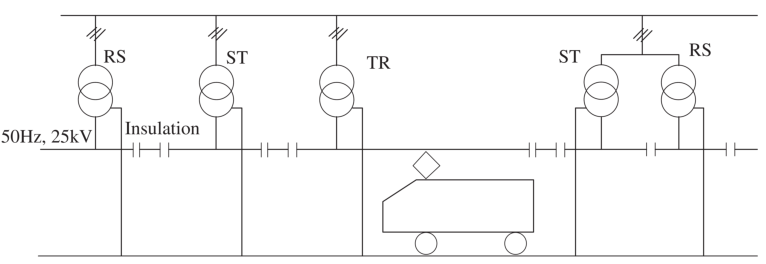
\includegraphics[width=\textwidth,keepaspectratio]{figures/31.PowerS/abad2016d}
		%		\vspace{2em}
		\captionof{figure}{6-pulse and 12-pulse diode rectifier configurations. Adapted from \cite{abad2016}.}
		\label{fig:abad2016d}
	\end{minipage}%
	\begin{minipage}{.03\textwidth}  ~\end{minipage}	
	\begin{minipage}{.45\textwidth}
		\centering
		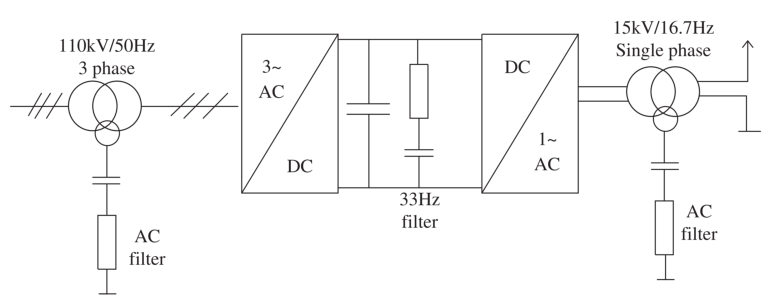
\includegraphics[width=\textwidth,keepaspectratio]{figures/31.PowerS/abad2016e}
		%		\vspace{0.5em}
		\captionof{figure}{DC supply system architecture. Adapted from \cite{abad2016}.}
		\label{fig:abad2016e}
	\end{minipage}
\end{figure}



\subsection{Train Power Supply System}
\label{subs:313}
In this subsection, three types of powering in trains are presented. The first two require a catenary to supply the train and the third are dependent on on-board energy generation (using diesel internal combustion engine).


\paragraph{1. DC supply system\\}


The DC catenary allows an almost direct connection between train power traction and inverter DC bus, as represented in figure \ref{fig:abad2016c}.

\begin{figure}[h!]
	\centering
	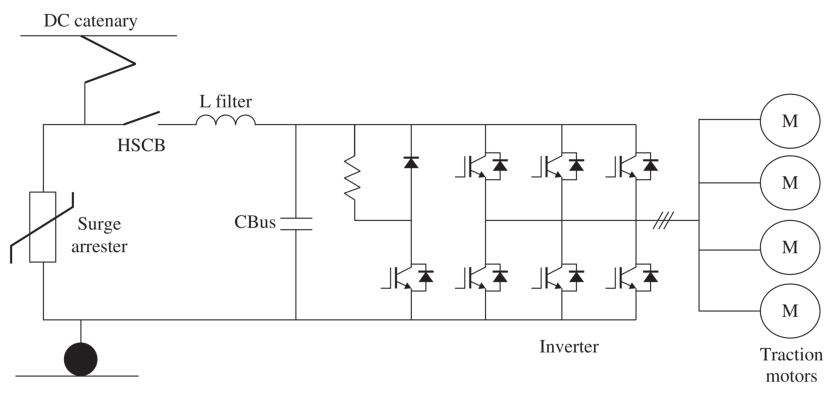
\includegraphics[width=0.65\textwidth,keepaspectratio]{figures/31.PowerS/abad2016c}
	\caption{Train internal power circuit of a DC supply system. Adapted from \cite{abad2016}.}
	\label{fig:abad2016c}
\end{figure}

\paragraph{2. AC supply system\\}

As previously presented, the catenary voltages can be either AC or DC. On the AC catenaries, a single phase transformer and an rectifier is needed to create a DC bus for traction power converters, as presented in figure \ref{fig:abad2016g}.


\begin{figure}[h!]
	\centering
	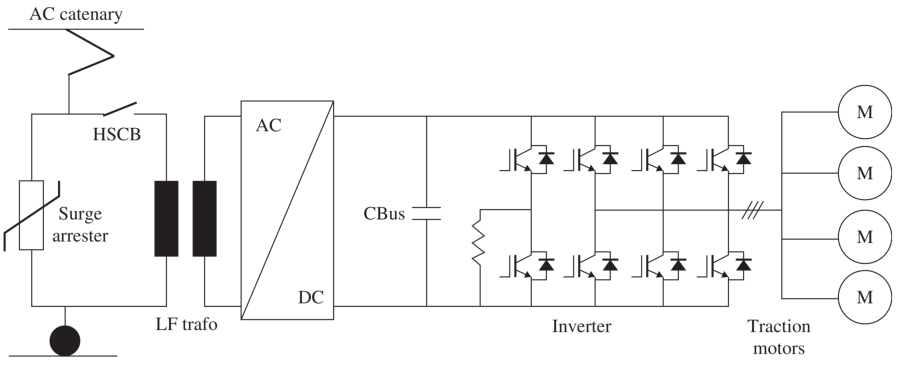
\includegraphics[width=0.65\textwidth,keepaspectratio]{figures/31.PowerS/abad2016g}
	\caption{Train internal power circuit of a AC supply system. Adapted from \cite{abad2016}.}
	\label{fig:abad2016g}
\end{figure}

\paragraph{3. Diesel-electric supply system\\}

An important market share in railway traction is occupied by diesel trains. This type of traction allows the avoidance of catenaries as the power source. The internal power circuit of those trains is presented in figure \ref{fig:abad2016h}.

\begin{figure}[h!]
	\centering
	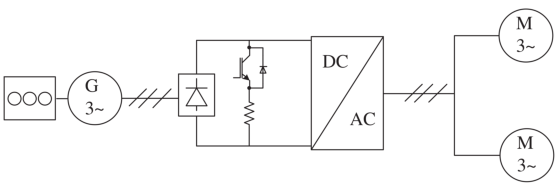
\includegraphics[width=0.55\textwidth,keepaspectratio]{figures/31.PowerS/abad2016h}
	\caption{Train internal power circuit of a Diesel electric locomotive with alternator. Adapted from \cite{abad2016}.}
	\label{fig:abad2016h}
\end{figure}


\subsection{Train Power Components}
\label{subs:314}
\paragraph{1.Pantograph\\}

	The pantograph is a device capable of maintain an electrical contact between train and catenary while in motion.
	
\paragraph{2.Surge Arrester\\}

	This equipment ensures over-voltage protection of train internal circuit, against external events (such as lightings) or internal events (switching faults)
	
\paragraph{3.High-speed Circuit Breaker\\}
	
	This device allows the safe interruption of high current faults.
	
\paragraph{4.Input LC filter\\}

	The main objective is to improve the power quality of the energy supply with the reduction of harmonic distortion (with the absorption of high frequency harmonics and injection of low frequency ones).

\paragraph{5.Filter inductor and DC-link capacitor\\}

	Coupled with electronic power converters/inverters, the filter inductor and DC-link capacitor allows the rectification of the AC voltage into DC. (?)
	
\paragraph{6.Power semiconductors\\}


\paragraph{7.Braking resistor\\}

	Avoid the occurrence of dangerous DC-link voltages (if the main AC grid does not support the generated energy)

\paragraph{8.Power converter box\\}

	Includes the power semiconductors (in power inverter arrangement) and cooling media.

\paragraph{9.Electric traction motor\\}

	Enables mechanical propulsion. The most common technology is the squirrel cage induction motor.



\newpage




\section{Section 2: Energy Sensors}


In this section is covered the theory behind energy sensors as well as the technologies used. In subsection \ref{subs:321} is started the presentation of the electric energy. Further on, in subsection \ref{subs:322} is covered the energy transducers and in subsection \ref{subs:323} is presented the challenges and requirements of energy measurement in RTS. 
%This section is concluded with the presentation of the technologies used in RTS for energy measurement purposes.

\subsection{Electric Energy Overview}
\label{subs:321}
Energy in form of electricity is the major traction player on the RTS. 
Complementary to the Diesel, this form of energy is distributed along with the rails in catenaries.
As presented in previous section, there are two major ways of rail electrification: AC or DC.

When a train is connected to a DC transmission line, it is possible to exchange energy from and to the catenary, complying to the Kirchhoff's circuit laws. The catenary is considered as a node that has multiple bi-directional power flow elements, specifically, trains and traction substations.

On AC transmission lines, the power flow is directly related to the relation between the voltage and current waveforms, as presented in figures \ref{fig:traction} and \ref{fig:generation}.

\begin{figure}[h!]
	\centering
	\begin{minipage}{.48\textwidth}
		\centering
		%		\vspace{2.5em}
			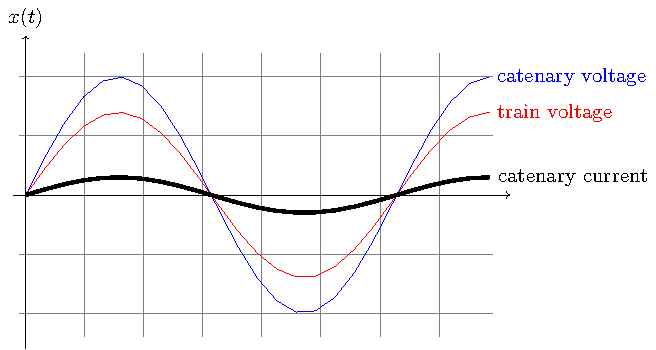
\includegraphics[width=1\textwidth,keepaspectratio]{figures/32.EnergyS/traction}
		%		\vspace{2em}
		\captionof{figure}{Waveforms in traction mode.}
		\label{fig:traction}
	\end{minipage}%
	\begin{minipage}{.01\textwidth}  ~\end{minipage}	
	\begin{minipage}{.48\textwidth}
		\centering
		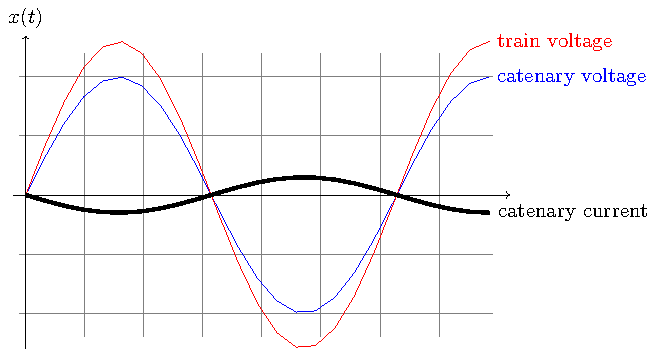
\includegraphics[width=1\textwidth,keepaspectratio]{figures/32.EnergyS/generation}

		
		%		\vspace{0.5em}
		\captionof{figure}{Waveforms in generation mode.}
		\label{fig:generation}
	\end{minipage}
\end{figure}

The energy calculation depends on the voltage and currents measured in the catenary. This function present in train energy meters evaluates the voltage and currents and generates the active, reactive and power factor information of the train. In figure \ref{fig:liran2014} is presented an example of the energy information 1h operation of {$HX_D1B$} locomotive.


\begin{figure}[h!]
	\centering
	\begin{minipage}{0.8\textwidth}
		\centering
				\vspace{-0.75em}
		\includegraphics[width=0.75\textwidth,keepaspectratio]{figures/32.EnergyS/liran2014}
				\vspace{-0.75em}
		\captionof{figure}{1h waveforms of active power (black), reactive power (red) and power factor (blue) of {$HX_D1B$} locomotive.  Adapted from \cite{liran2014}.}
		\label{fig:liran2014}
	\end{minipage}%
	
\end{figure}


\subsection{Current transducers and voltage transducers}
\label{subs:322}	
	According to \cite{webster2012}, a transducer is a device capable to convert different physical signal forms. In the scope of energy measurements, current and voltage transducers are employed. These devices converts the field energy waveforms into a voltage (or current) waveform capable of be acquired by a processing unit (such as a microcontroller, PLC, etc).
	
	\cite{Dalessandro2007} identifies multiple different physical effects associated to the current sensors\footnote{In the scope of energy measurements, voltage transducers combine the measurement of a current in a given load (or resistor). Therefore this subsection will only cover the measurement of currents} as following:
	
	\begin{description}
		\setlength\itemsep{-0em}
		\item [Magnetic coupling] Using the knowledge of transformers, it is possible to perform isolated current measurements. The current transformers are widely used in energy measurement and are based on the magnetic coupling concept, with a ferromagnetic core. With the same magnetic coupling principle, the Rogowski coil is a helix wound around a non-magnetic torus and uses the magnetic coupling physical effect to measure the current, as the integrative of the induced voltage on coil terminals;
		%5-7
		\item [Magneto resistance] The anisotropic magneto-resistive current sensors uses a magneto-resistive sensing element (composed of a nickel iron alloy) to measure the magnetic field induced by a current on a conductor;
		%8,9
		\item [Faraday induction] Fiber optic current sensors relies on Faraday effect to integrate the magnetic field along the closest path. The magnetic field will cause a magnetooptic phase shift of the light waves and this phase shift is measured with a technique known as fiber gyroscopes;
		%10
		\item [Hall Effect] Similarly to magneto-resistive current sensors, the hall effect sensors uses a sensing element to measure the magnetic field in the air-gap of a magnetic circuit. For AC-only current measurement, no compensation of the flux in the magnetic core is made. The implementation of "Zero flux" compensation avoids the saturation of the magnetic core. This active compensation allows the measurement of currents with DC component.
		
	\end{description}

	The voltage transducers depends of an indirect measurement of the electric field. In particular, the principle is the combination of the current measurement in a known load (or resistor), connected to the terminals of the circuit intended to be measured and using the principles previously presented in 
	

\subsection{Energy measurement in RTS}	
\label{subs:323}

	Currently, the European Commission requires the implementation of mechanisms in RTS for energy liberalization, where the Railway Undertakings (RUs) can purchase energy from suppliers of their choice, \cite{eur-lex2008}.
	
	The impact of such requirement is the liberalization of the energy market, which brings new challenges in the railway sector. In practical, on-board energy metering is important to make energy savings visible and to allocate the profits of these savings to the respective RUs.
	
	As an example, EcoS energy meter for railway, presented in figure \ref{fig:ecos}, identifies the following requirements to comply with:
	
	\begin{description}
	\setlength\itemsep{-0em}
	
	\item [EN 50463 standard \cite{EN50463}] This standard defines the architecture of the Energy Measurement System. It is composed by two blocks: (1) the Energy Measurement Function, responsible for the measurement of voltage and current and for the calculation of the energy and (2) the Data Handling System, that joins the timestamp and the GPS location to the energy data. In section \textit{3.4: Smart Metering}, the components of this standard are better described;
	
	\item [EN 50155 standard \cite{EN50155}] This standard defines the aspects of temperature, humidity, shock, vibration, and other parameters that covers electronic equipment used on rolling stock for railway applications;
	
	\item [AC and DC measurement channels] The energy meter comply with multiple catenary topologies;
	
	\item [Multiple Connectivity] EcoS uses WiFi, Ethernet and 2G/3G/4G. In addiction it is used the localization and time sync from GPS and Train Communication \& Management System (TCMS);
	
	\item [Multiple access and customization] EcoS implements web interface and a SoftPLC for expansions and customizations.
	\end{description}



\begin{figure}[h!]
	\centering
	\begin{minipage}{.8\textwidth}
		\centering
		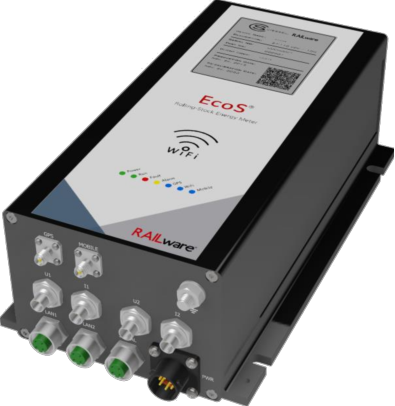
\includegraphics[width=0.35\textwidth,keepaspectratio]{figures/32.EnergyS/ecos}
		%		\vspace{0.5em}
		\captionof{figure}{EcoS railway energy meter. Adapted from railware.it}
		\label{fig:ecos}
	\end{minipage}
\end{figure}


\subsection{Energy measurement function}
\label{subs:324}

With the compliment of the EN50463 standard, the EcoS energy meter performs the energy calculations as presented in figure \ref{fig:energy_calculation}.

\begin{figure}[h!]
	\centering
	\begin{minipage}{.8\textwidth}
		\centering
		\vspace{-0.5em}
		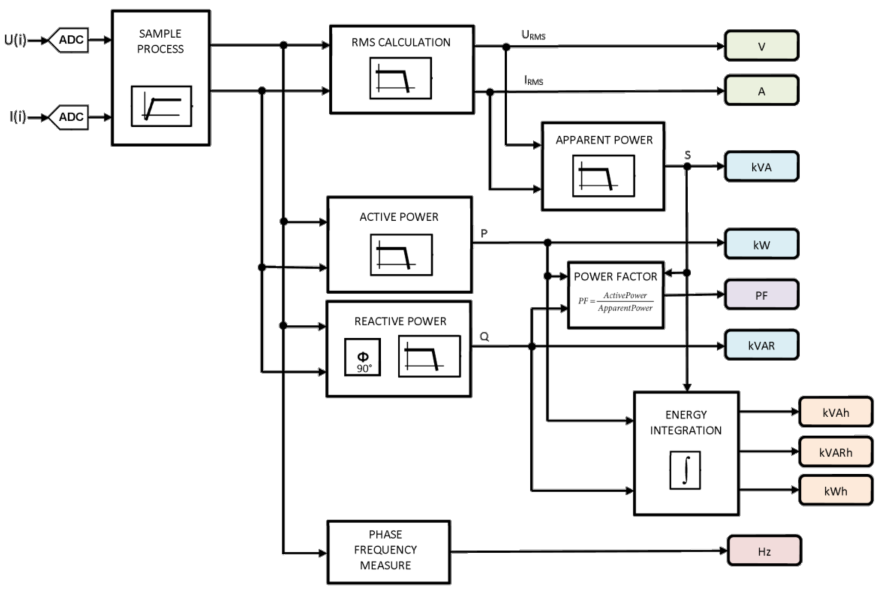
\includegraphics[width=\textwidth,keepaspectratio]{figures/32.EnergyS/energy_calculation}
		%		\vspace{0.5em}
		\captionof{figure}{EcoS power calculation function. Adapted from railware.it}
		\label{fig:energy_calculation}
				\vspace{-1em}
	\end{minipage}
\end{figure}

\begin{comment}


\subsection{Energy measurement technologies in RTS }
\label{subs:324}



\begin{figure}[h!]
	\centering
	\begin{minipage}{0.40\textwidth}
		\centering
		%		\vspace{2.5em}
		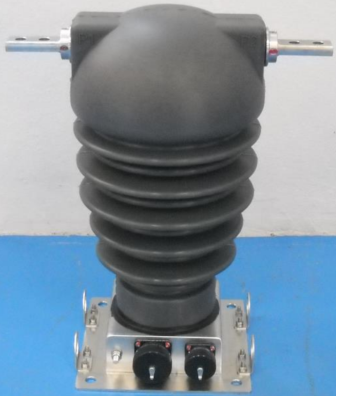
\includegraphics[width=0.75\textwidth,keepaspectratio]{figures/32.EnergyS/current_t}
		%		\vspace{2em}
		\captionof{figure}{25 kV current transformer. Adapted from ?}%\footnotetext{www.railware.it}}
		\label{fig:current_t}
	\end{minipage}%
	\begin{minipage}{0.05\textwidth}  ~\end{minipage}	
	\begin{minipage}{0.40\textwidth}
		\centering
		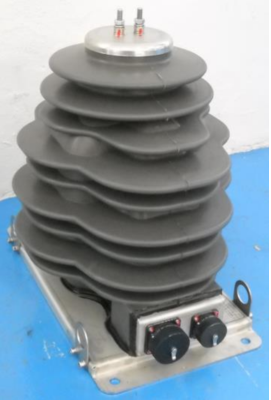
\includegraphics[width=0.59625\textwidth,keepaspectratio]{figures/32.EnergyS/voltage_t}
		
		
		%		\vspace{0.5em}
		\captionof{figure}{25 kV voltage transformer. Adapted from ?}%\footnotetext{www.railware.it}}
		\label{fig:voltage_t}
	\end{minipage}
\end{figure}

\end{comment}



\newpage





\section{Section 3: Wireless networks}

In this section, communication networks are presented, with special attention to wireless technologies. An historic overview is presented 



1.	Network technologies – historic overview

2.	Current technologies and standards:

3.	Emerging technologies and standards

4.	Network Simulators and Network Emulators






\subsection{Network technologies – historic overview}

The beginning of modern communication systems is marked with the expansion of the telegraph, having an important milestone happening in 1858 with the first communication between USA and UK. Since then, the telephone has emerged and widely used; the wireless communication was successfully established in 1901 and, decades later, worldwide communication had the support of satellite communication systems.

One important area of communications is the computer networks, and in particular, the internet where it is used in several aspect of business (such as advertising, production, shipping, planning, billing, and accounting, \cite{comer2008}). In 1980 the Internet was a research project involving few dozen sites and currently the Internet is an important part of people’s communication.

Currently, a computer network is well organized, having a well structured Internet Protocol (IP) that defines how data passes through layers, as represented in figure \ref{fig:comer2008}.

	\begin{figure}[h!]
	\centering
	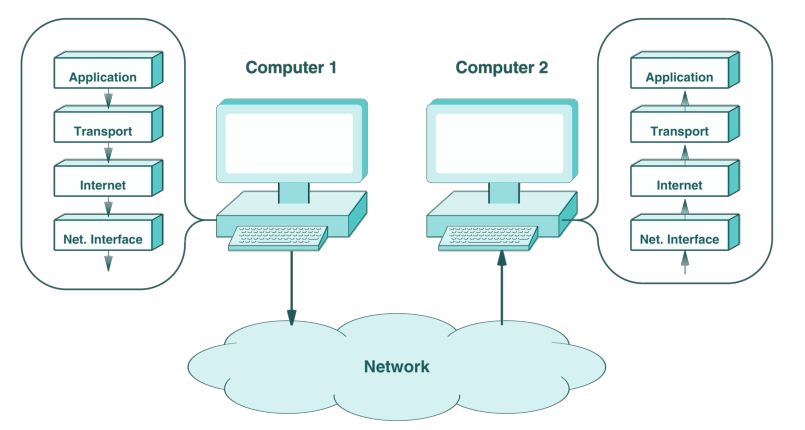
\includegraphics[width=0.8\textwidth,keepaspectratio]{figures/33.WirelessN/comer2008}
	\caption{Representation of data flow in a computer network. Adapted from \cite{comer2008}.}
	\label{fig:comer2008}
\end{figure}


\subsection{Current Wireless technologies and standards}

The following sections will cover the wireless communications in smart metering systems, starting with the low-rate and low-power communications applied on smart meters and ending with the high-rate communications (and consequently higher costs and power than low rate communications). With the increasing on demand for higher bandwidth, broadband technologies such as mobile WiMAX, IEEE 802.16e and broadband PLC are expected to be considered and used in newer installations, \cite{Mohassel2014}.


%As the demand for bandwidth increases, broadband technologies such as IEEE 802.16e, mobile WiMAX and broadband PLC are going to play a key role in newer installations, \cite{Mohassel2014}.

\subsubsection{IEEE 802.11 (Wireless LAN (WLAN) or Wi-Fi)}

IEEE 802.11 is the standard for the information exchange between systems and for the telecommunications. The coverage area of this technology is on local and metropolitan area networks (LANs and MANs). The specific requirements are on the Medium Access Control and on Physical Layer. The most popular versions of this standard is the IEEE 802.11b and IEEE 802.11g, that differs in the modulation technique (Direct Sequence Spread Spectrum (DSSS) technique versus Orthogonal Frequency Division Multiplexing (OFDM) modulation technique). The data rates are, respectively, 11 Mbps and 54 Mbps, \cite{Usman2013, ieee2012}.



\subsubsection{IEEE 802.15.4 (ZigBee)}

The standard IEEE 802.15.4 imposes conditions in the physical layer and media access control focusing on low-rate (up to 300 kHz) wireless personal area networks. Developed by the Zigbee Alliance and covering the specifications of the IEEE 802.15.4 on the physical layer and the medium access control, Zigbee is a commonly used for low power wireless communication technology. It operates on the ISM bands of 868 MHz, 915 MHz and 2.4 GHz adopting direct sequence spread spectrum (DSSS), \cite{Usman2013}.

%IEEE 802.15.4 is a standard that specifies the physical layer and media access control for low-rate (up to 300kHz) wireless personal area networks. ZigBee is a popular, low power wireless communication technology developed by the ZigBee Alliance based on the Physical Layer and Media Access Control Layer of the IEEE 802.15.4 standard.
%It operates on the ISM bands of 868 MHz, 915 MHz and 2.4 GHz adopting direct sequence spread spectrum (DSSS), \cite{Usman2013}.


\subsubsection{DASH7}

On the low-rate field of research, an alternative to Zigbee is the DASH7. Using the ISO/IEC 18000-7 standard to support this wireless sensor network technology, DASH7 is developed to reach active Radio Frequency Identification Devices (RFIDs) and operates at 433MHz band. The advantage is the typical range of 250m (could achieve 5 km) and has a typical and maximum data rates of 28 kbps and 200 kbps, being in this specifically designed for Smart Grid and for applications in Smart Energy.


\subsubsection{6LoWPAN}

This IETF development group promotes specifications for the usage of IPv6 on IEEE 802.15.4 networks. It allows the connection between low-power devices to IP networks, with the usage of fragmentation and compression of messages. In conclusion, 6LoWPAN creates an adaptation layer between the IEEE 802.15.4 and IPv6.



\subsubsection{Wibree}

This wireless communication technology is designed for low power consumption and short-range communication. It is designed to work with Bluetooth and, the Bluetooth-Wibree depends on the existing Bluetooth RF and allows ultra-low power consumption.


\subsubsection{Industrial Wireless Communications: WirelessHART and ISA100.11a}

Launched by HART Communication Foundation in September of 2007, WirelessHART is an open wireless communication standard designated specifically for the process measurement and control applications, \cite{Song2008}. This standard is specifically designed to comply with industrial requirements, such as stricter timing requirement, higher security concern, immunity to harsher interferences and obstacles and enough scalability to be used in large process control systems.

Similarly, ISA100.11a aims to provide secure and reliable wireless communication for noncritical monitoring and control applications, \cite{Petersen2011}.





\subsubsection{IEEE 802.16 (WiMAX)}

On the field of the broadband wireless communication there is the Worldwide Interoperability for Microwave Access (WiMAX) under the IEEE 802.16 standard. It is specifically developed aiming the point-to-multipoint communications being applied in fixed and mobile applications and it has data rates up to 70 Mbps over a distance of 50 km. Framed into the smart grid systems, this communication technology is considered as a solution for high data rate communication link to be applied at the backbone of the utilities, \cite{Usman2013}.


\subsubsection{Broadband communications: GSM/GPRS and LTE/LTE-Advanced}

Operating at 900 MHz and 1800 MHz, the Global System for Mobile communications (GSM) is the most used cellular network all over the world. The modulation technique is the Gaussian Minimum Shift Keying (GMSK) and it achieves transfer rates up to 270 kbps. Its architecture consists of four components: the Operation Support Substation, the Network Switching Substation, the Base Station Subsystem and the Mobile handset. Due to its level of development around the world being present in remote locations, this advantage makes this  an interesting technology to be applied in Smart Grid applications, \cite{Usman2013}.

Long Term Evolution (LTE) is a recent standard for wireless technology that allows high data rates with high capacity and low latency and with a good Quality of Service (QoS). The improved version of this technology, the LTE-Advanced, admit higher capacity with expanded peak data rate of 1 Gbps for the downlink and 500 Mbps for the uplink, obtained on the increase of the spectral efficiency, higher  number of active subscribers connected at the same time, and better performance at cell edges, \cite{Mohassel2014}. This technology, for the Smart Metering environment where the high bandwidth and good QoS are mandatory at some communication points.


\subsection{Protocols and standards}
%\lipsum[4]

In computer networks, a protocol is a set of rules that ensure a communication of specific set of information between two machines. A standard is a document that specifies several aspects of something that has the overwhelming agreement and support of an entity (the standards making body). In the networking area, several protocols are supported by standards. In this section is presented some of the protocols that ensure a coherent communication among the sensor networks.

\subsubsection{IEEE 802.15}

The standard family defines the topologies and network roles. In particular, it defines the physical (frequency and channels, spectrum handling, modulation and bit rate) and MAC (packet formats, operational modes, timing aspects, topologies) layers of the OSI model (\cite{Hackmann2006}).


\begin{figure}[h!]
	\centering
	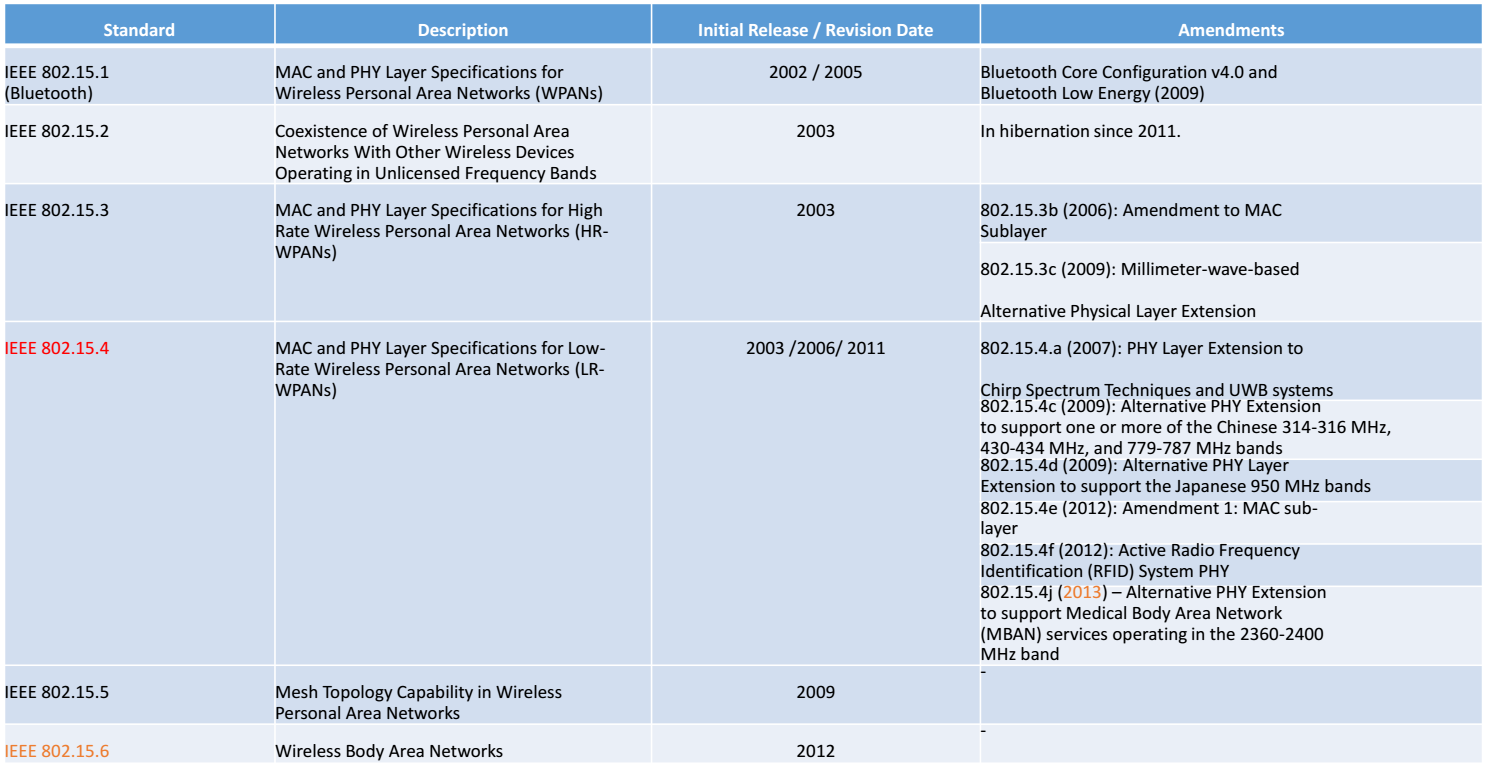
\includegraphics[width=1.1\textwidth,keepaspectratio]{figures/nancy2014}
	\caption{Members of the 802.15 family. Adapted from \cite{nancy2014} lecture presentation slides.}
	\label{fig:nancy2014}
\end{figure}

Based on figure \ref{fig:nancy2014}, the 802.15.4 is the standard that defines the PHY and MAC layers for low rate wireless personal area networks. It supports \textbf{full-function devices} (device capable of being the network coordinator or simple node and can have implemented complex network functionalities) and \textbf{reduced-function device} (limited devices with low-bandwidth limitations and limited or no-network intelligence). The possible network topologies are the following:

\begin{description}
	\item[Star ---] Each device in the network communicates with the full-function device network coordinator;
	
	\item[Peer-to-peer ---] All devices communicate with each other (if they are in the communication range). Sufficiently flexible to implement more complex topologies such as multi-hoping, cluster trees and mesh topologies;
	
	\item[Multi-hopping ---] This is a technique that allows the usage of two or more wireless nodes to convey data from a source to a destination;
	
	\item[Cluster trees] Topology to reduce the routing complexity where each node knows its parent node and all it's child nodes. It has always only one single path between two nodes.
	
	\item[Wireless mesh] This technique allows data to be propagated along a path by hopping from node to node until it reaches its destination.
	
\end{description}

\subsubsection{802.15.4-based wireless standards}

\cite{Radmand2010} presents a comparison of wireless sensor standards for industrial applications. In figure \ref{fig:radmand2010} is present the overall schema of the wireless standards.


\begin{figure}[h!]
	\centering
	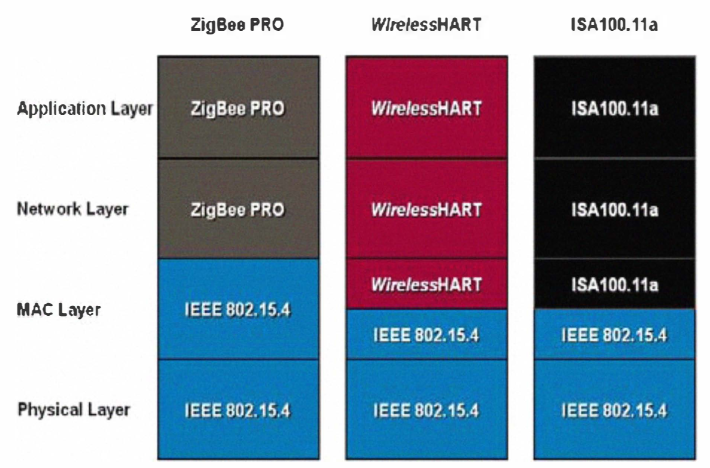
\includegraphics[width=0.6\textwidth,keepaspectratio]{figures/radmand2010}
	\caption{Overall schema of wireless standards. Adapted from \cite{Radmand2010}.}
	\label{fig:radmand2010}
\end{figure}


\subsection{Communication KPI’s}
%\lipsum[4]

According to \cite{Radmand2010}, it is identified the following "Industrial Requirements" for the WSN's:

\begin{description}
	\item[Reliability ---] Reliability is a measurement of the transmission accuracy, in percentage, that evaluates the amount of data that reach its destination. This measurement uses the properties of data communication, acknowledge-based usually.
	
	\item[Latency ---] Latency is the measurement of the time delay and is defined as the time that a data packet takes to be transmitted from the source to the destination. The latency is directly related to the link quality and a high latency link is result of a link with high signal-to-noise ratio. 
	
	\item[Sensor Data Update Rates ---] This KPI is not directly related with the communication link. However the update rate of the sensor data affects the power consumption due to the increase of the processing effort. In a SYNC-based update rate, this KPI is related to the frequency of the SYNC event.
	
	\item[Wireless Transmission Range ---] This KPI is the maximum distance that a communication link supports the data transfer with a given reliability and in specific conditions (indoor/outdoor; line-of-sight or LOS).
	
	\item[Power consumption ---] The power consumption is a measurement of the combination of the computational effort of the nodes and the transmission effort. It is directly related with the update rate as well as with the link quality and, if it exists, the routing activity in each node.
	
\end{description}

%\subsection{Emerging Technologies and Research Trends}

%%ver livro khan

\subsection{Network Simulators and Network Emulators}


In this subsection is covered the network simulators. The usage of network simulators allows the modeling of various scenarios of real environment. However, pure network simulators avoids the interaction with real environment, which leads space for network emulators, as a hybrid method to combine simulation capabilities with hardware and software components of real networks. Therefore, in this subsection is referred the simulators that allows integration with hardware and software network components, to have an overview on the network emulators.

In figure \ref{fig:simul_VS_emul} is presented the framework on the mechanisms to evaluate the performance of networks.

\begin{figure}[h!]
	\centering
	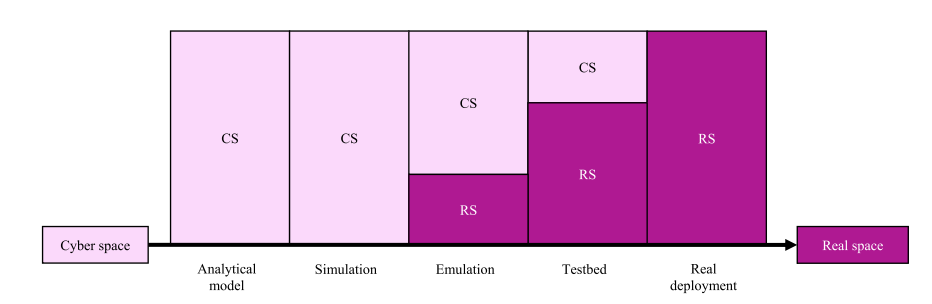
\includegraphics[width=1\textwidth,keepaspectratio]{figures/simul_VS_emul}
	\caption{Simulation \& emulation framework.}
	\label{fig:simul_VS_emul}
\end{figure}

An extensive review on simulation tools, made by \cite{nayyar2015}, is presented as following:

\begin{description}
	\setlength\itemsep{0.5em}
	%%1
	\item [NS-2 (network simulator-2)] 
	Object orientated discrete event simulator tool, based on two languages (C++ and OTcl). 
	
	%%2
	\item [NS-3 (network simulator-3)] 
	Written in pure C++, this simulator has been extensively explored in the literature with various modules like 802.15.4, 6LoWPAN and RPL available. With the usage of ns-3 in emulation mode, the implementation of real testbeds can be validated since it is possible to generate repeatable experimental results, with the usage of real-world network environment that includes all of the ns-3 tracing, logging, visualization and statistics gathering tools.
	
	%%3
	\item [OMNET++] 
	This simulator is based in C++ in the basic modules and uses Network DEscription (.NED) scripts to connect and assemble the simulation basic modules.

	%%4
	\item [J-Sim] 
	JavaSim Simulator has been developed in Java and it has several advantages to carry out large scale WSN simulations.

	%%5
	\item [Mannasim] 
	Is based on NS-2 to perform WSN simulations.

	%%6
	\item [SensorSim] 
	Similarly to Mannasim, this is a framework for WSN based on NS-2 simulator. However it is not available, currently, to the public. 

	%%7
	\item [NRL Sensorsim] 
	This extension to NS-2 simulator is focused on WSN, similarly to SensorSim and Mannasim frameworks. Currently, it is no longer in development and does not have support.

	%%8
	\item [NCTUns 6.0] 
	On the field of network emulators, this software has the main advantage of using the real world Linux TCP/IP stack and implements almost every IEEE network standards. Last release was on 2010.

	%%9
	\item [SSFNet] 
	Java simulator designed especially for WSN's. Last release in 2004.

	%%10
	\item [GloMoSim] 
	Non-commercial simulator (the commercial version is \textit{"QualNet"}) designed for wireless and wired network systems.

	%%11
	\item [QualNet 7.0 + EXata 5] 
	Considered one of the most advanced simulator platform these days, QualNet enables a high fidelity virtual model of network, with an advanced GUI. It has a free academic version.

	%%12
	\item [sQualNet Simulator] 
	Is an extension of QualNet for sensor network specific models. 

	%%13
	\item [OPNET Modeler Suite] 
	Is a powerful collection with an interactive GUI to build network scenarios. It has a free academic edition. 

	%%14
	\item [SENSE] 
	Is a powerful sensor network simulator and emulator.

	%%15
	\item [DRMSim] 
	Is a Java-based software that enables large-scale network simulation.

	%%16
	\item [NetSim] 
	Is a simulator designed for protocol modeling, network research and development and defense applications.

	%%17
	\item [UWSim] 
	This simulator is designed for marine robotics research.

	%%18
	\item [Visual Sense] 
	This modeling and simulation software is designed for wireless and WSN applications, as an extension of Ptolemy II.

	%%19
	\item [Viptos] 
	Is an interface/bridge between TinyOS and Ptolemy II.

	%%20
	\item [PTOLEMY II] 
	Is an open source simulation software, based on Java and with actor-oriented design (where actors are software components, have a concurrent execution and communicate via interconnected ports)
	
	%%21
	\item [SENS] 
	This specific framework for WSN's simulator and emulator that uses a simplified sensor model.
	
	%%22
	\item [SHAWN]	
	Is a customizable sensor network simulator focused on the simulation of the effect caused by a phenomenon (not the phenomenon itself) with scalability and support for extremely large networks. According to SHAWN development repository, last contribution was on 2013.
		
	%%23
	\item [SIDnet-SWANS]
	This Java-based simulator was made to provide a simulation and proof-of-concept platform for application of WSN's.
	Latest version was released in 2011.
	
	%%24
	\item [WSim/Worldsens Simulator/WSNet Simulator]
	This simulator states for being an event-driven simulator for large scale wireless networks. Latest version was released in 2009.

	%%25
	\item [WSN Localization Simulator]
	This is a WSN location simulator stating for being easy, scalable and extendable to many/different localization schemes. It was released in 2013.
	
	%%26
	\item [NetTopo Simulator]
	This framework is an open source simulator designed in Java. Its main objective is to analyze various algorithms in WSN's. 
	
	%%27
	\item [SIDH]
	Is a Java-based simulator focused on the simulation of thousand of sensor nodes.
	
	%%28
	\item [PROWLER]
	The Probabilistic Wireless Sensor Network Simulator is a framework that runs under Matlab and is focused to TinyOS applications.
	
	%%29
	\item [Matlab/Simulink]
	With extensive usage by the research community, Matlab and Simulink software provides resourceful toolboxes for simulation of communication networks, being possible to build a complete WSN model system.
	
	%%30
	\item [PiccSIM]
	This simulation platform uses Matlab/Simuling and NS-2 for networked control systems (in particular wireless)
	
	%%31
	\item [LabVIEW]
	Various toolboxes to simulate WSN's are available with LabVIEW.
	
\end{description}


\subsubsection{Evaluation of network tools}

In the previous list, several tools for the evaluation of network performance was presented. Special attention is given for the tools that has large support either for implementation of several network technologies (wired and wireless) and, with this requirement, the following network simulators will be considered for further research:
	
\begin{itemize}
	\setlength\itemsep{-0.5em}
	\item NS-3;
	\item OMNET++;
	\item QualNet 7.0 + EXata 5;
	\item MatLab Simulink;
\end{itemize}




\newpage




\section{Section 4: Smart metering}

In this section, special attention is given to smart metering. The smart grid framework is presented to justify the need for smart meters and then, an overview on metering systems is presented.


1.	Smart grids and the need for smart meters

2.	Metering systems – overview

3.	Metering systems in railways

4.	Wireless sensor networks – overview

5.	Smart metering with WSN in Railway Transportation System (RTS)

\subsection{Smart grids and the need for smart meters}

Smart Grids improves the functionality and concept of traditional electrical grids by obtaining the grid component's data using Information and Communication Technology (ICT). Such grids benefit the reliability and the efficiency of the system with the usage of the acquired data, \cite{Mohassel2014}.

Although the smart meters does not have an effective definition, those devices are composed by an electronic box and a communication link, \cite{Seppo2012}. A smart meter is responsible for measuring the energy-related parameters and the user consumption with a given time interval. All those measurements are then transmitted upon a communication network to the utility or to other player with the responsibility of using the meter data. The information obtained from the data is shared with consumer-side devices, to inform the end-users on their related costs and energy usage, \cite{Siano2014}.

Smart meters implement a bidirectional communication on top of AMR. They are inherent to smart grid systems. 

Similarly to the evolution of electricity meters, the utility grid has evolved from a centralized production and control perspective to a distributed one. The conventional electrical grid is a network with a transmission link connecting power producers and end-user consumers. The control and distribution of electrical power is made in a centralized way. With the increase of power demand, increase of complexity and having more and more decentralized power generation, a migration to the smart grid framework is required, \cite{Reddy2014}.

\subsection{Features of Smart Meters and metering systems}

A smart metering system combines several controlling devices, a extensive number of sensors for measuring the parameters and devices responsible for the transferring of the data and the commands. The detection of unauthorized consumption due to electrical energy theft and the improvement of the energy in the distribution are other advantages of smart meters. These devices acts as a gateway by having a communication interface protocol to the database stored by the utility company, \cite{Reddy2014}.

The design of an ideal smart grid has to focus on prediction, adaptability and reliability points. Moreover, it requires to cover the demand adjustment, the load handling, flexibility and sustainability and it should incorporate advanced services. In advance, an end to end control capability has to be ensured as well as finding the optimal cost and asses, increase the quality of energy and quality of service. Another features of smart grids are the automatic restoration ans self-healing, being all the previously presented features of the smart grids highly dependent of the role of the smart meters, \cite{Mohassel2014}.

Smart-meter types are also distinguished based on features like data-storage, communication type and connection with the energy supplier. The data storage capability allows data to be stored in the meter, being transferred after a few days or weeks to the Meter Data Management System (MDMS) of the utility. Compensations for some power quality deficiencies can be also considered; therefore the future meters should be also capable of register certain basic power quality characteristics. In advance, the design of rate and tariffs of electricity providers determine the requirements such as the period of meter intervals or the temporal resolution (commonly ranging from 15 min to 1 h). During those intervals, the production and consumption of active and reactive power is mandatory to be separately measured, \cite{Siano2014}.

\subsection{Metering systems in railways}

Towards na increase of interoperability of the rail system within the Community \cite{eur-lex2008}, the Directive 2008/57/EC specifies the need of Technical Specifications for Interoperability (TSIs), presenting essential requirements in which each rail subsystem should meet to ensure the interoperability of the railway system within the EU. Those TSIs are of the responsibility of European Union Agency for Railways (ERA) and are listed as following:

\begin{itemize}
	\setlength\itemsep{-0.5em}
	\item Locomotives and passenger rolling stock - 1302/2014;
	\item Noise - 1304/2014;
	\item Wagons - 321/2013;
	\item Infrastructure - 1299/2014/EU;
	\item Energy - 1301/2014;
	\item Control command and signalling - 2012/88/EU;
	\item Persons with reduced mobility - 1300/2014/EU;
	\item Safety in railway tunnels - 1303/2014;
	\item Operation and traffic management - 2015/995/EU;
	\item Telematics applications for freight service - 1305/2014/EU;
	\item Telematics applications for passenger service - 454/2011;
		
\end{itemize}


On the energy field and with the purpose of implementing on-ground energy data collecting systems (data collecting service - DCS), technical specifications for interoperability relating to the ‘energy’ subsystem of the rail system in the Union are specified in the Commission Regulation (EU) No 1301/2014, \cite{eur-lex2014}. 



The On-Board energy measurement systems are pointed in Appendix D of Commission Regulation (EU) No 1302/2014 \cite{eur-lex2014b}. This regulation appendix presents the requirements for such energy measurement system. The general architecture is defined as following:

\begin{itemize}
	\setlength\itemsep{-0.5em}
	\item \textbf{Energy measurement function (EMF)}, measuring the voltage and current, calculating the energy and producing energy data;
	\item \textbf{Data handling system (DHS)}, producing compiled energy billing data sets for energy billing purposes, by merging data from the EMF with time data and geographical position, and storing it to be sent to on-ground data collection system (DCS) by a communication system;
	\item \textbf{On-board location function}, giving geographical position of the traction unit. Contrary to fixed installation revenue meters, train meters must have the knowledge of time and geographical position \cite{metas2015};
\end{itemize}

Figure \ref{fig:EMS} presents the general overview of the on-board energy measurement system.

\begin{figure}[h!]
	\centering
	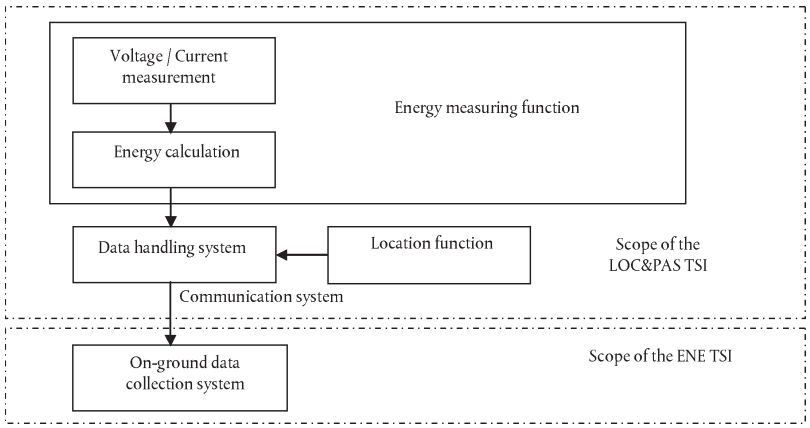
\includegraphics[width=0.85\textwidth,keepaspectratio]{figures/EMS}
	\caption{Functions, data flow and regulation scope of on-board energy measurement system.}
	\label{fig:EMS}
\end{figure}

As global requirements, all active and reactive energy should be measured, the measurement equipments should be rated to match the traction unit current and voltage rating, the system should be protected from intrusion, and finally, the loss of power in the  measurement system should not affect the data stored in EMS.

Complementary to the previously presented system requirements, each component of the energy measurement system has specific requirements as listed as following:

\begin{description}
	\setlength\itemsep{-0.5em}
	
	\item [Energy measurement function (EMF)] Has specific metrological requirements to specify the accuracy of the sensors and it has the requirement of having the reference period of 5 minutes defined by the UTC clock time (shorter measuring period is allowed in the case that the data is aggregated into 5 minutes time reference period);
	
	\item [Data handling system (DHS)] Should compile the data (without corrupting them), using the same time reference as EMF. This system should store compiled data of, at least, 60 days' continuous work and should have an alternative method of accessing the data. Finally, this system should produce compiled energy billing data sets (CEBD) by including an EMS identification number, a timestamp, a location data and the consumed/regenerated active and reactive energy.
	
	\item [Location function] Has specific location requirements to define the latitude and longitude, as well as a accuracy of 250m and the location data information should have the same timestamp.
	
	\item [On-board to ground communication] The specification related to interface protocols and transferred data format are an open point.
	
\end{description} 


 \cite{metas2015} lists the standards that should be considered to the certification of Energy Measurement Systems on on-board trains:
 
 \begin{description}
 	\setlength\itemsep{-0.5em}
	\item [EN 50463-1] General;
	\item [EN 50463-3] Data Handling System;
	\item [EN 50463-4] Communication;
	\item [EN 50463-5] Conformity Assessment.
 \end{description} 




%\subsection{Wireless sensor networks – overview}


\subsection{Smart metering with WSN in Railway Transportation System (RTS)}


%%%%%%%%%%%%%%%%%%%%%%%%%%%%%%%%
%%%%%%%%%%%%%%%%%%%%%%%%%%%%%%%%%
%%%%%%%%%%%%%%%%%%%%%%%%%%%%%%%%%
\newpage




\section{Section 5: Decision Support Systems (DSS)}

1.	Overview/definition
2.	Eco-driving – driving assistant
3.	Timetable scheduling
4.	Maintenance support
\newpage


\section{Section 6: Issues and problems in WSN}
An important contribution of a wireless sensor network in the railway system is the availability of useful knowledge about energy consumption to the decision support systems.

Therefore, such acquisition systems are required to provide accurate data regardless of the quality of the acquisition sensors, \ac{EMI}, sensor supply fluctuations, among other error sources.

Through computational algorithms, the increase of communication reliability and fault tolerance is possible. Those computational algorithms detect outliers or, in the scope of this PhD, detect erroneous data that will disturb the outcomes of decision support systems. 



\subsection{Outlier and outlier detection}

\label{sec:def}
Outlier detection is a computational task to detect and retrieve information from erroneous data values. The definition is usually close to anomaly detection or deviation detection. 

\cite{class:branch:2006} identifies outlier detection as an essential step to either suppress or amplify outliers and precedes most data analysis routine. \cite{nn:abid:2016} points the need of detecting aberrant data and sensors within an \ac{WSN}. \cite{nn:zhuang:2006} extends the outlier definition to the case where the outliers are introduced in sensing queries and in sensing data analysis.

%%%%%%%%%%%  outlier defnition in the scope of my phd
\vspace{1em}

In the scope of the PhD, an outlier is a data value or a data instance that do not represent the correct consumption status.

The threshold of what is an outlier or not (or a value that do represent the correct consumption status or not) is given by the output of the subsystem that is immediately after the acquisition of consumption status subsystem, the decision support subsystem, gave a correct output or not. Figure \ref{fig:general} illustrates the integration of the consumption acquisition subsystems with the decision support subsystem.


\begin{figure}[h!]
	\centering
	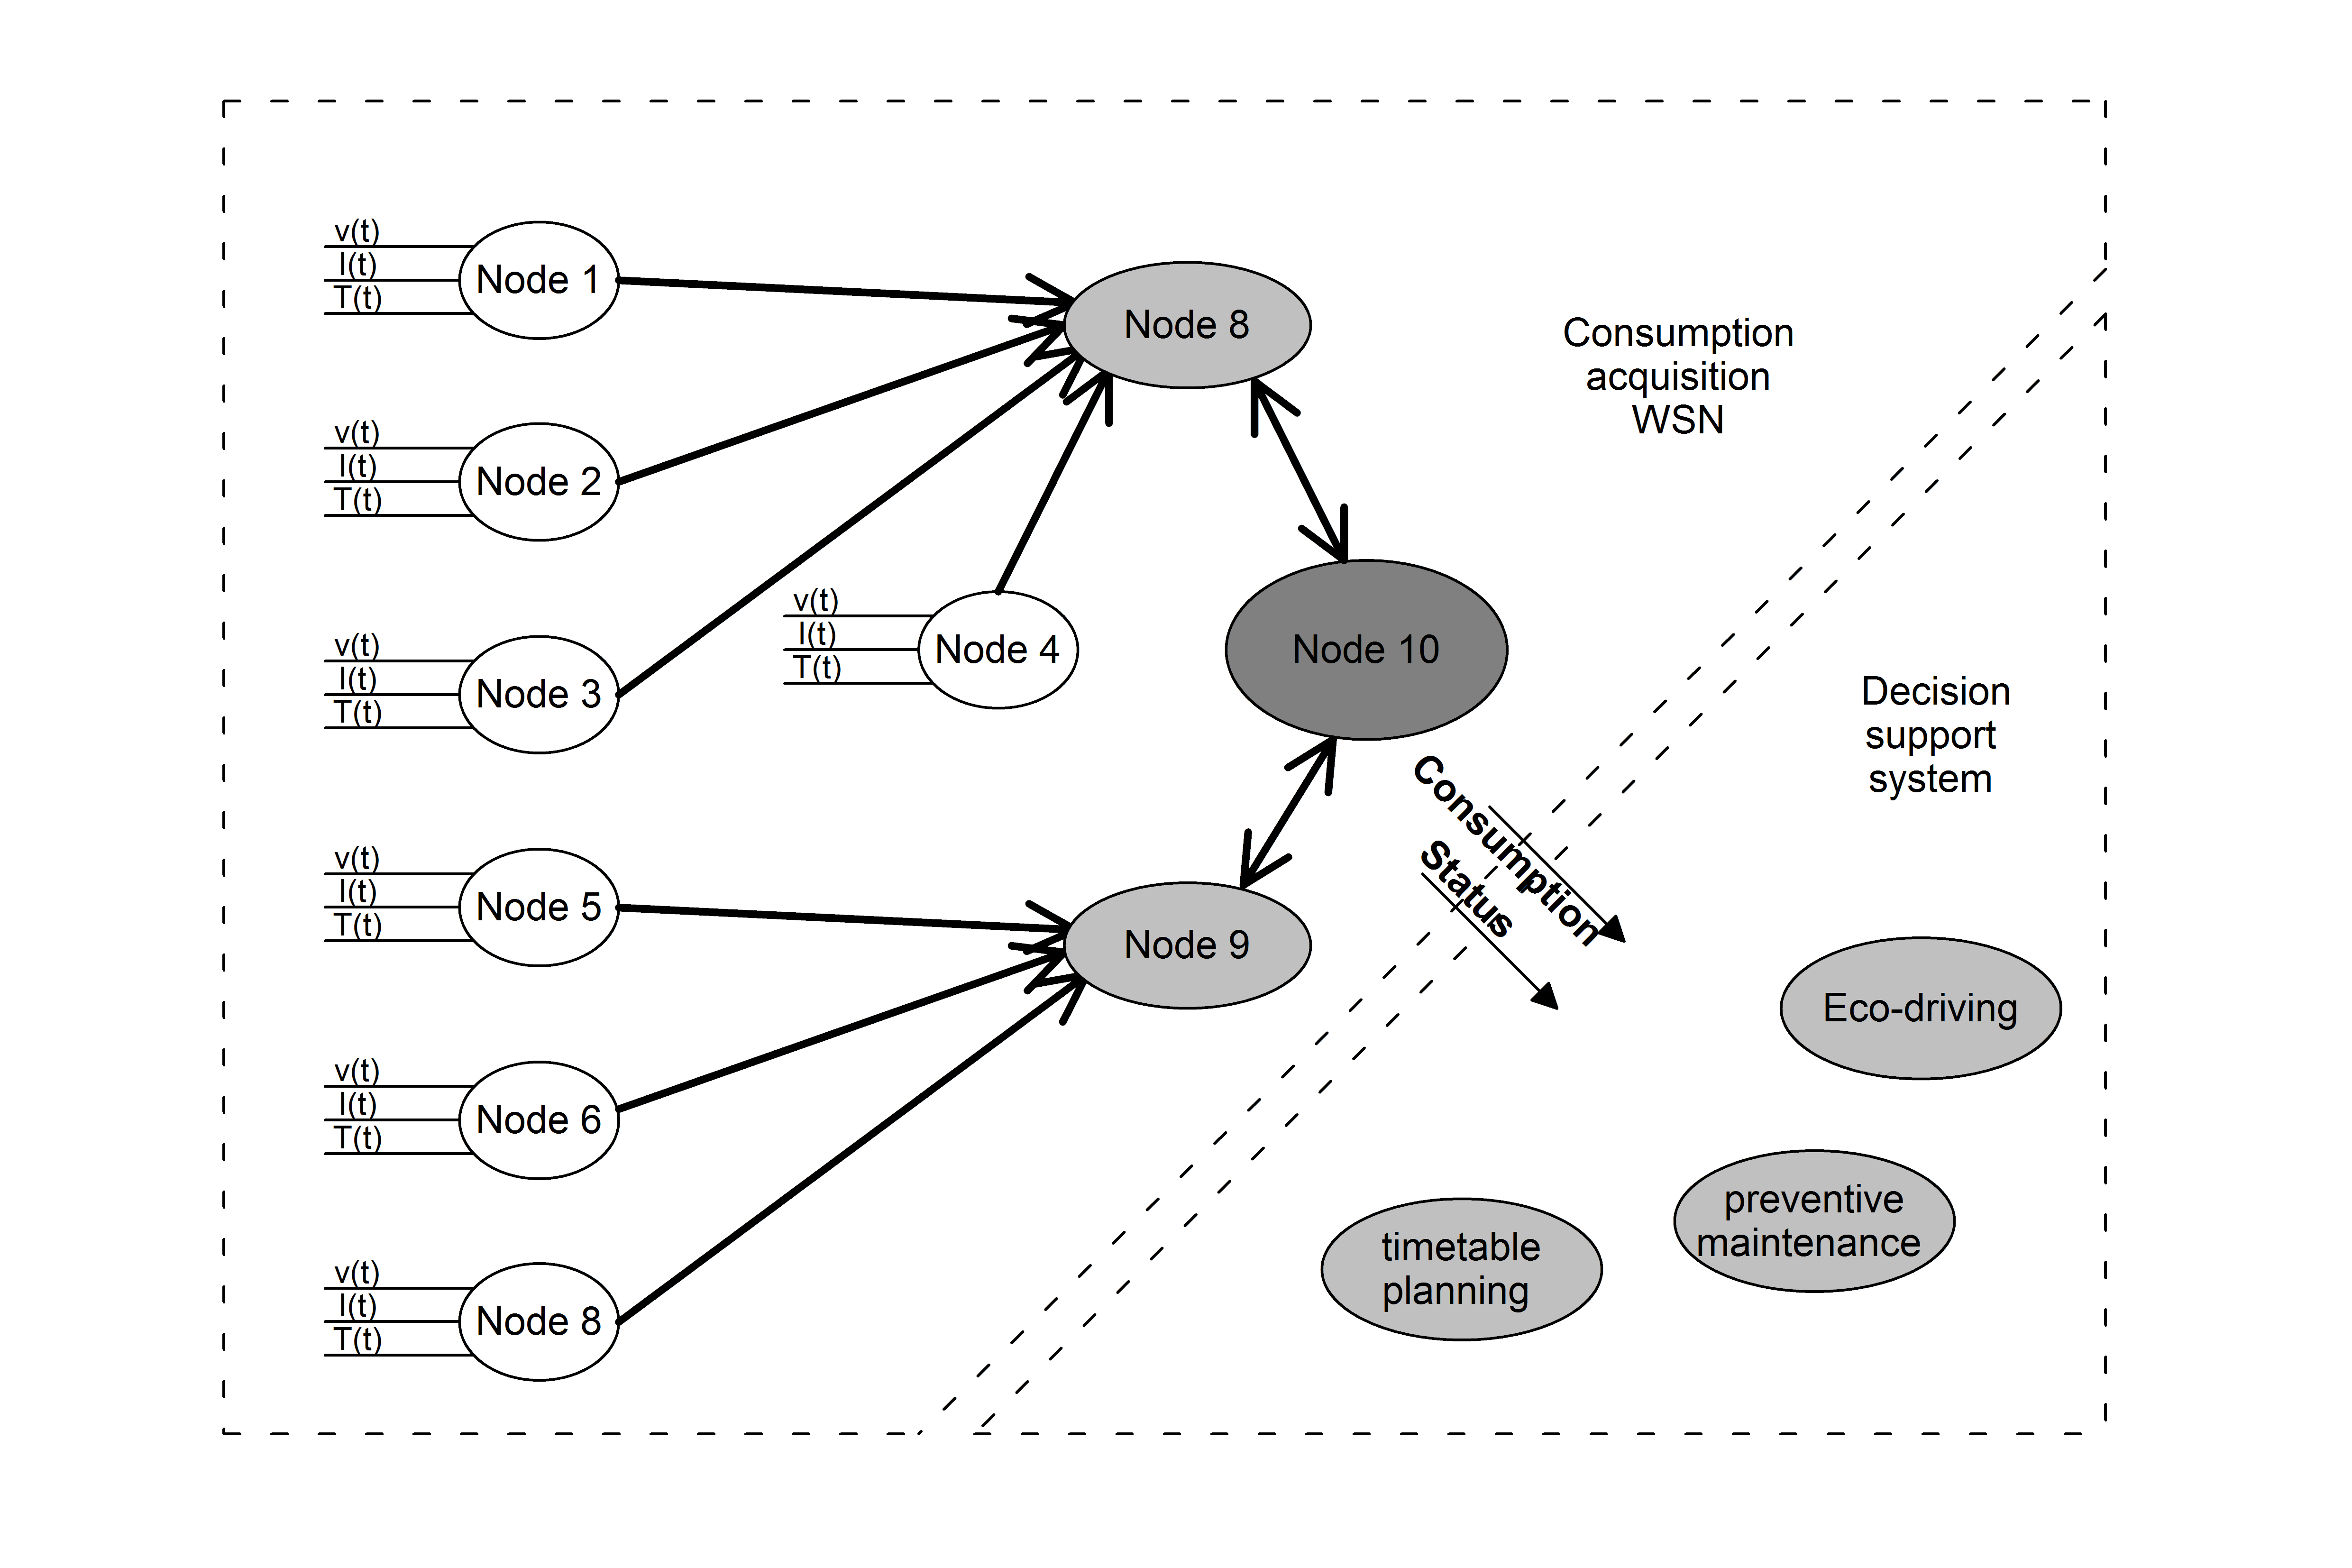
\includegraphics[width=0.75\textwidth,keepaspectratio]{figures/general}
	\caption{Integration of the \ac{WSN} with a decision support system. }
	\label{fig:general}
\end{figure}

\newpage
Without an outlier detection mechanism, the decision support subsystem may have the following outputs:


\begin{description}
	\setlength\itemsep{-0.5em}
	\item[Input deviation from real value lower than a threshold]
	The Decision Support Subsystem output is in accordance to the real consumption conditions.
	\item[Input deviation from real value greater than a threshold]
	The Decision Support Subsystem output is not in accordance to the real consumption conditions.	
\end{description}

The problem of taking decisions based on wrong considerations of the consumption status is that it may lead to loss in desirable efficiency or increase of costs.

Let us consider a simple and hypothetical example where the \ac{DSS} will provide an output towards suggesting an action in preventive maintenance based on the usage of a component. Considering that the usage of the component is depending on the counting of situations that the component is working above the nominal conditions. Without an outlier detection mechanism, the outliers will induce the \ac{DSS} in counting situations of overcharge of the component, where the measurement is not related to working nominal conditions but is related to external influences, such as \ac{EMI} or temperature. The output of \ac{DSS} may suggest a preventive maintenance on a component that is working in proper conditions.

To conclude, with an outlier detection mechanism in the consumption acquisition subsystem the decision support subsystem may know if the value of consumption is an outlier or not and, with that information, the \ac{DSS} output will be more accurate with the real conditions of operation.


\subsection{Literature review of Outlier detection in \ac{WSN}}
\label{sec:od_wsn}
\ac{WSN} has been widely used in several applications in several domains such as industrial, scientific, medical and others. Those applications have been supported by the advances in wireless technologies as well as in the evolution of microcontroller technologies, with enhanced processing capabilities associated with reduced energy consumption.

\subsubsection{Motivation}

\cite{class:rajasegarar:2007} points an important motivation for the inclusion of computational algorithms, i.e. outlier detection algorithms, to reduce the transmission of erroneous data, since in WSNs, the majority of the energy consumption occurs in radio communication. In particular, they present the case of Sensoria sensors and Berkeley motes, where the energy consumption in communication exceeds, in ranges from 1000 to 10000, the energy consumption of computation.

Thus, this raises a research opportunity to reduce the communication usage of $\mu C$s, by adding processing features, where the small increase in the computation will significantly reduce the energy consumption in the transmission. These processing features are, among others, the outlier detection algorithms.


On the field of the quality of the data acquired by \ac{WSN}, the motivation of detecting outliers in data acquired from \ac{WSN} has been extensively presented in the literature. The need for acquire data from harsh or "highly dynamic" environments as well as the need to validate and extract knowledge from the acquired data are one of the main points in the motivation to study the outlier detection in \ac{WSN},  \cite{gen:zhang:2010,gen:chandola:2009,stat:ghorbel:2015,class:martins:2015b}.



\subsubsection{Research areas}
Zhang et al. \cite{gen:zhang:2010} identifies the outlier detection research areas in three domains: 

\begin{itemize}
	\item Intrusion detection: Situation caused by malicious attacks, where the detection techniques are query-driven techniques;
	
	\item Fault detection: Situation where the data suffer from noise and errors and where the detection techniques are data-driven ones;
	
	\item Event detection: Situation caused by the occurrence of one atomic or multiple events and where the majority of the research has been developed due to its complexity.
\end{itemize}

Based on the division of this three domains, the upcoming research is intended to be focused on the event detection and fault detection techniques. Specifically, the main goal for this research will be the event detection algorithms.


\subsubsection{Challenges}

The challenges of outlier detection in WSNs are related to the quality of the acquisition of the sensors, the reliability of the modules in terms of energy or environmental susceptibility, and the communication requirements and restrictions.

Zhang et al. \cite{gen:zhang:2010} lists the challenges as the following:

\begin{itemize}
	\setlength\itemsep{-0.5em}
	
	\item Resource constraints;
	
	\item High communication costs;
	
	\item Distributed streaming data;
	
	\item Dynamic network topology, \\ frequent communication failures, \\ mobility and heterogeneity of nodes;
	
	\item Large-scale deployment;
	
	\item Identifier outlier sources;
	
\end{itemize}

\cite{class:branch:2006} identifies an important challenge, where the probability of occurrence of outlier events are extremely small. \cite{nn:abid:2016} as well as \cite{stat:sheng:2007} identifies the large amount of data as the main challenge for outlier detection in WSN. \cite{nn:zhuang:2006} identifies the inexpensive and low fidelity sensors as the main reason for the error generation and the main challenge is identified on the distributed streaming data among a large amount of sensors. \cite{stat:ghorbel:2015} points the main challenge as the processing of data from sensors that generate continuously data, that is uncertain and unreliable. 

To conclude, the main challenge will be the usage of inexpensive and low fidelity sensors that will be affected by the rush railway environment. Complementary, the main challenge of using outlier detection mechanisms in the railway \ac{WSN} is the balance between the detection accuracy and the influence that undetected data-instances will induce in other subsystems (in particular in decision support systems dependent on data from the \ac{WSN}). In addition, the detection accuracy is directly related with the memory usage, computational requirements, communication overhead, etc. 


\subsection{Taxonomy of Outlier Detection Techniques}
\label{sec:taxon}
The study of detection techniques requires a well-defined taxonomy framework that addresses the related work on the different areas. This taxonomy is well defined and solid in the literature, where the works of \cite{gen:zhang:2010} and \cite{gen:chandola:2009} reflect a similar approach on presenting a taxonomy for outlier detection techniques.

In the following sections, a coverage in relevant techniques is presented:

\begin{itemize}
	\setlength\itemsep{-0.5em}
	\item Classification based techniques.
	\subitem Bayesian Networks
	\subitem Rule-based techniques
	\subitem Support Vector Machines
	
	\item Statistical based techniques.
	\subitem Parametric --- Gaussian based
	\subitem Non-parametric --- Histogram based
	\subitem Non-parametric --- Kernel function based
	
	\item Nearest Neighbor-based techniques.
	\subitem Using distance
	\subitem Using relative density
	
	\item Clustering based techniques.
	
	\item Spectral Decomposition based techniques.
	
\end{itemize}

\begin{comment}


\subsection{Classification based techniques}
\label{sec:classbased}

Classification based techniques are based on systematic learning approaches which use sets of data. 
The supervised approaches require previous knowledge to train a model (or classifier) from a set of data instances (or training data) and classifies a new data instance as normal or as outlier. 
The unsupervised approaches do not require knowledge and learn the boundary around normal instances, declaring the new instance as normal or as outlier depending if the data instance is outside of the boundary of the previous data sets.

The classification based techniques are listed as the following:

\begin{itemize}
	\setlength\itemsep{-0.5em}
	\item Neural Networks-based;
	\item Bayesian Networks-based;
	\item Rule-based;
	\item Support Vector Machines-based.
	
\end{itemize}

\vspace{0.5em}

Neural networks-based approaches are interesting strategies for outlier detection where a given neural network might be trained with only normal data-sets. 
At testing stage, the data instances that are similar to the training data-set are accepted by the neural network and then considered as normal. 
The remaining data-sets are rejected by the neural network due to their lack of similarity with normal data-sets. Thus, those data instances are considered as outliers. 
%Based on the table \ref{table:t3}, t
These techniques are classified as semi-supervised due to their need for normal data-sets for the training stage.

\vspace{0.5em}

Bayesian networks-based approaches are identified as prominent techniques for outlier detection in WSNs, being the reason why they are extensively covered further on in \ref{subsec:bay}.
Those techniques use probabilistic graphical models to detect outliers based on the interdependencies of different variables.

\vspace{0.5em}

Rule-based techniques, presented in \ref{subsec:rule}, classify an outlier based on a confidence value related to the number of the training instances correctly classified by a given rule and the total number of training instances covered by the same rule. For each test instance, all the rules are tested and the confidence value is ordered. The output of this outlier detection technique is given by the inverse of the confidence value of the rule that better captures the test instance.

\vspace{0.5em}

Support Vector Machine (SVM) techniques are used for outlier detection to classify a given instance based on the fitness of a hyper-sphere to the data in a higher dimensional space. 
The hyper-sphere is obtained with a linear optimization algorithm where the objective function of this linear optimization problem is to minimize the radius R that cover the majority of the image vectors. The output of the SVM applied to OD is the classification of the image vectors as outliers if they are outside of the hyper-sphere. The SVM techniques are presented in \ref{subsec:svm}.
\subsubsection{Bayesian Networks}
\label{subsec:bay}
\cite{gen:zhang:2010} divide the bayesian network based techniques in three categories: 

\begin{itemize}
	\setlength\itemsep{-0.5em}
	\item Na\"{i}ve Bayesian Networks;
	\item Bayesian Belief Networks;
	\item Dynamic Bayesian Network Models;	
\end{itemize}

All those approaches use probabilistic graphical models to represent a set of variables and their probabilistic interdependencies. 
This graphical model aggregates the information from different variables and provides an estimate on the expectancy of an event to belong to the learned class.

\cite{class:xiang:2016} illustrates an application to measure the concentration of NO$_2$, CO and O$_3$ pollutants, using a bayesian network. All the three variables are all correlated and also depends on the temperature as presented in figure \ref{fig:xiang2016}. The real measurements acquired by the microcontroller are represented with (s) and the representations in (t) refers to the real concentration of those pollutants.

\begin{figure}[h!]
	\centering
	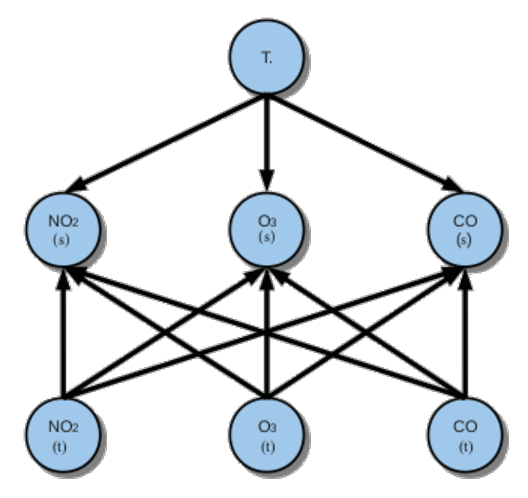
\includegraphics[width=0.60\textwidth,keepaspectratio]{figures/xiang2016}
	\caption{Application of a Bayesian Network to an atmospheric measurement system. }
	\label{fig:xiang2016}
\end{figure}

The three categories presented by \cite{gen:zhang:2010} differs between them where the first category captures the sensor nodes correlations on spatio-temporal domain; 
The second one considers not only the spatio-temporal correlations but also the conditional dependence of sensor attributes;
The third category proposes the measurement of state variables at a current time instance.

\cite{class:janakiram:2006} proposes the detection of outliers in sensor streamed data by capturing the conditional dependencies among the observation of it's attributes. this is made in three phases:

\begin{description}
	\setlength\itemsep{-0.5em}
	\item[Training Phase]  
	Phase where the Bayesian Belief Network is trained to capture the spatio-temporal correlations.
	\item[Testing Phase]  
	Phase where the trained BBN is tested on the level of accuracy and, if needed, the learned parameters are updated.
	\item[Inference Phase] 
	Phase where the missing values are inferred and the remaining streamed data are tested to detect if it is an outlier or not.
\end{description}

\cite{class:janakiram:2006} also defined the BBN, where the BBN is a directed graph, together with an associated set of probabilistic tables.
The graph is divided in nodes and arcs, where the nodes represents the variables and the arcs are the representation of the casual/influential relationship among variables.

The main contribution of BBN is the possibility to have a model that, with the dependency between uncertain variables (by filling a node probability table), it is possible to describe complex probabilistic reasoning about uncertainty.

\cite{class:janakiram:2006} describes their process in three steps:

\begin{itemize}
	%\setlength\itemsep{-0.5em}
	
	\item Constructing the Bayesian Belief Network
	\subitem \textbf{IF} a few variables have direct dependencies
	\subitem \textbf{AND} many of the variables are conditionally independent
	\subitem \textbf{THEN} all the probabilities can be computed from the joint probability distribution.
	
	\item Learning Bayesian Belief Networks
	\subitem \textbf{IF} the network structure is given
	\subitem \textbf{AND} all variables are fully observable in the training examples
	\subitem \textbf{THEN} estimating the conditional probabilities is enough
	\subitem
	\subitem \textbf{IF} the network structure is given
	\subitem \textbf{AND} some of the variables are observable
	\subitem \textbf{THEN} apply neural network using Gradient Ascent Procedure
	\subitem
	\subitem \textbf{IF} the network structure is unknown
	\subitem \textbf{THEN} Use heuristic search
	\subitem \textbf{OR} Use constraint-based technique to search through potential structures
	
	
	\item Inferring from Bayesian Belief Networks
	\subitem \textbf{THESIS} The probability distribution of certain attributes might be inferred
	\subitem \textbf{PROOF} Given the fact that the values that other attributes can take are known	
\end{itemize}

\cite{class:paola:2015} proposes an adaptive distributed Bayesian approach for detecting outliers in data collected by a WSN.
The focus of the proposed algorithm is the optimization of outlier classification accuracy, time and communication complexity and also considering externally imposed constraints on conflicting goals. The proposed algorithm is intended to run in each sensor node. 

From the individual sensor node point of view, this algorithm consists in two phases:

\begin{description}
	\setlength\itemsep{-0.5em}
	\item[Outlier detection]  
	Where, based on sensor readings and on the collaboration with neighbors, is made the probabilistic inference where the results are evaluated in three metrics: classification accuracy, time complexity and communication complexity.
	
	\item[Neighborhood selection] 
	Where the best neighbors are identified and selected to cooperate with, and, in addiction, to correspond to a reconfiguration of the Bayesian Network structure.
\end{description}

In the global point of view, if there is a high number of cooperating nodes, the classification is naturally higher with the drawback if increasing the processing time and communication complexity (thus resulting in increased detection delay and increase of energy consumption).

\cite{class:xiang:2016} proposes the addition of recover and recalibrate the drifted sensors simultaneously based on the usage of a Bayesian network. 
The authors have applied their algorithm to the measurement of the variables in the sensor readings of the NO$_2$, CO and O$_3$ pollutants, as previously presented in figure \ref{fig:xiang2016}.
Based on the correlations of the sensor readings and on the temperature influence, the algorithm itself detects the outliers, recover valid information and adjust the BBN to automatically recalibrate the sensor.




\subsubsection{Rule-based techniques}
\label{subsec:rule}
Rule based is another classification based technique for outlier detection. Similarly, this technique is based on a training stage from a data-set and a model generation to detect new data-instances based on history values.

Rule based techniques depends on two steps \cite{gen:chandola:2009}:

\begin{itemize}
	%\setlength\itemsep{-0.5em}
	\item \textbf{1. Learn rules from the training data-set}\\
	Using a learning algorithm (i.e. RIPPER, Decision Tree, etc.)\\
	Where each rule has an associated confidence value 	proportional to the ratio:\\
	{\centering	$\text{\footnotesize Confidence Value} = \frac{\text{number of training instances correctly classified by the rule}}{\text{number of total training instances covered by the rule}}$
	}
	
	\item \textbf{2. Find for each test instance the rule}\\
	That better capture the given test instance.
	
	\item \textbf{$\Rightarrow$ The anomaly score is}\\
	The inverse of the confidence value for the rule that better capture the test instance.
	
\end{itemize}

\cite{class:islam:2016} proposes an algorithm for outlier detection inserted in rule-based taxonomy. They propose a new belief-rule-based association rule, with the focus on handling various types of uncertainties. 

Due to the nature of the sensor data, a traditional inference mechanism cannot be used. Therefore, they propose a new inference mechanism for the rule-based algorithm that consists of an input transaction database that is converted into the following:
\begin{itemize}
	\setlength\itemsep{-0.5em}
	\item belief transaction database;
	\item support calculation;
	\item belief matrix;
	\item confidence calculation;
	\item belief association rule discovery.
	
\end{itemize}


%\newpage
\vspace{1.5em}

\subsubsection{Support Vector Machines}
\label{subsec:svm}
Rather than performing outlier detection in the central node, \cite{class:rajasegarar:2007} proposes a 
distributed approach to:

\begin{itemize}
	\setlength\itemsep{-0.5em}
	\item performs detection on local data at each node
	\item and communicates to the parent node only the summary information to perform at upper layer the global classification of the data.	
\end{itemize}

Their proposal is based on a one-class quarter sphere SVM and is divided into 2 parts:

\begin{itemize}
	\setlength\itemsep{-0.5em}
	\item \textbf{Anomaly detection  algorithm}
	\subitem The OD is supported by previous works where, with the fitness approach of a hypersphere to the data in a higher dimensional space, and by applying a linear optimization to the problem of fitting the hypersphere with minimal radius R, having the center fixed at the origin and encompassing the majority of the image vectors.
	\subitem The result of the linear optimization problem is the classification of the image vectors as:
	
	\vspace{-1em}
	
	\subitem  \textbf{$\rightarrow$ Support Vectors}, if inside the sphere;
	\subitem  \textbf{$\rightarrow$ Outliers}, otherwise.
	\vspace{1em}
	
	\item \textbf{Distributed anomaly detection}
	\subitem \textbf{1$^{st}$ step:} Each sensor node runs the entire AD algorithm on local data;
	\subitem \textbf{2$^{nd}$ step:} The resulting radius is sent to the parent node;
	\subitem \textbf{3$^{rd}$ step:} Each parent computes the global radius;
	\subitem \textbf{4$^{th}$ step:} Parents sends the radius to children nodes;
	\subitem \textbf{5$^{th}$ step:} Children compares global radius with local one and updates parameters.
	
\end{itemize}


\cite{class:xu:2012} proposes a KNN-SVM which is a Support Vector Machine based on K-Nearest Neighbor Algorithm.

Despite KNN taxonomy is presented further on in \ref{sec:nnbased}, in a synthesis  the KNN is a distance-based approach that detect outliers in data-instances lying in the sparsest regions or lying in the outside of a given model boundary of the feature space.

Considering the Quarter sphere SVM technique proposed by \cite{class:rajasegarar:2007} the KNN-SVM combine the origin and the radius R that contain most of the samples and introduces kernel functions to make the optimization region more tighten. 

\subsection{Statistical based techniques}
\label{sec:statbased}



\cite{gen:chandola:2009} identifies the statistical techniques for anomaly detection based on the assumption that, in a stochastic model, the most common data instances occur in high probability regions and the anomalies occur in low probability regions.

To detect anomalies, parametric techniques are suggested, since those techniques \textbf{assume} the knowledge of the underlying distribution and \textbf{estimate} the parameters from a given data set. Non-parametric techniques differ from parametric ones without the need of assuming the knowledge of the distribution.

\cite{cluster:andrade2016} lists some statistical parametric techniques: 

\begin{description}
	\setlength\itemsep{-0.5em}
	\item[Peirce's Criterion]  
	This statistical parametric method is based on a normal distribution.
	\item[Chauvenet's Criterion]  
	Is based on the assumption that a given arbitrary measurement may be rejected, if the probability of having the deviation for the average value is lower than the inverse of the double of the number of measurements. 
	
\end{description}

\subsubsection{Parametric --- Gaussian based}
\cite{gen:zhang:2010} summarizes parametric techniques as an anomaly detection strategy based on the following steps:

\begin{itemize}
	\setlength\itemsep{-0.5em}
	\item The available knowledge is generated from a known distribution;
	\item The distribution parameters is then estimated from the given data.	
\end{itemize}

The usage of Gaussian  models allows the spatial correlation of readings towards distinguishing between outlying sensors and event boundary. 

\subsubsection{Non-parametric --- Histogram based}
\cite{stat:sheng:2007} proposes a histogram-based method to reduce the communication cost on sensor networks. The main objective of this proposal is to collect hints (in a form of histogram) about the data distribution and, with the knowledge from these hints, unnecessary data is filtered and potential outliers are detected 


Complementary, \cite{stat:wang:2013} introduces clusters on incremental histogram scheme based on a divide and conquer strategy:

\begin{itemize}
	\setlength\itemsep{-0.5em}
	\item The wireless network is divided in clusters (based on adjacent nodes and data correlated strategy);
	\item The cluster head and cluster members updates the histogram incrementally and compares histograms in the form of Kullback-leibler divergence differentially (Kullback-leibler divergence is a convenient and robust
	method of measuring the difference between two data sets in a
	statistical sense.)
\end{itemize}

%%%%%%%%%%%%%%%
%%%%%%%%%%%%%%%
\subsubsection{Non-parametric --- Kernel function based}
\cite{gen:zhang:2010} synthesizes the concept of Kernel function non-parametric approaches as methods for estimating the probability distribution function for normal instances (and a new instance that occurs on a low probability area is declared an outlier). Later on in section \ref{sec:specbased} is presented the Kernel Principal Component Analysis (KPCA) used by \cite{stat:ghorbel:2014} for outlier detection in WSN's.

\cite{cluster:andrade2016} identify some kernel regression techniques: 

\begin{description}
	\setlength\itemsep{-0.5em}
	\item[Marzullo's Fault Tolerant Sensor Averaging (FTA) ] 
	Simple method for sensor fusion where the data assumed as anomalous is deleted.
	\item[Elmenreich's Confidence-Weighted Averaging (CWA) ] 
	The sensor's confidence are correlated with the sensor's variance.
	\item[CWA+FTA method ]
	This method combines both methods where the confidence-weighted average is calculated and two-thirds of the anomalous data is removed.
\end{description}


\subsection{Nearest Neighbor-based techniques}

\label{sec:nnbased}



A promissory technique is extensively explored in the literature with the concept of neighborhoods, based on the key assumption that normal instances occurs in dense neighborhoods and anomalies occurs far from their closest neighbors.





\subsubsection{Using distance}



\cite{class:branch:2006} proposes algorithms that implements nearest neighbor-based techniques for outlier detection in WSN's. The proposed unsupervised anomaly detection techniques use the following different algorithms:



\begin{itemize}
	
	\setlength\itemsep{-0.5em}
	
	\item The distance to the $k^{th}$ nearest neighbor;
	
	\item The average distance to the k nearest neighbors;
	
	\item the inverse of the number of neighbors, within a distance $\alpha$.	
	
\end{itemize}



\cite{nn:abid:2016} bases the detection technique on the distance between the current measurement and its neighbors. A synthetic database is generated based on the insertion of random values into a real database (in particular the Intel Berkeley lab WSN database).

The procedure is divided in two steps: 

\begin{itemize}
	
	\setlength\itemsep{-0.5em}
	
	\item \textbf{Step 1a)} For a given time-slot, the data values are sorted in a vector;
	
	\item \textbf{Step 1b)} After that, for a given point in the vector, Euclidean distance between the predecessor and successor is calculated and stored in a second vector;
	
	\item \textbf{Step 1c)} Based on the smallest distance between the current point and the predecessor or successor, the current point is linked;
	
	\item \textbf{Step 2} If the point in the vector is not linked (due to its distance between current point and predecessor/successor higher than a threshold), is declared an outlier;
	
\end{itemize}





\subsubsection{Using relative density}

\cite{gen:chandola:2009} defines the NN technique using relative density as a technique that estimates the density of the neighborhood of all data instances. Depending if the instance corresponds to a dense neighborhood or a low density one, the data is declared as outlier or normal.

\subsection{Clustering based techniques}
\label{sec:clustbased}
%\lipsum[4-4]

\cite{gen:chandola:2009} synthesizes the clustering techniques in three categories based on three different assumptions: 

\begin{itemize}
	
	\setlength\itemsep{-0.5em}
	
	\item The normal data instances are part of a cluster in the data and the outliers does not fit any cluster;
	
	\item The normal data instances are present close to its closest cluster centroid and the outliers lies far away from their closest cluster centroid;
	
	\item The normal data instances are part of large dense clusters and the outliers are part of small or sparse clusters.
	
\end{itemize}

\cite{clust:rajasegarar:2006} uses a technique to minimize the communication overhead by using clusters among the sensor readings. In a further step, it merges the clusters before the data is sent to other nodes.

\cite{cluster:andrade2016} presents a methodology to apply clustering and statistical techniques. The clusters are grouped according to the spatial position of the sensors and a k-means nearest-neighbor technique is used to provide a better understanding of the sensed environment. The proposed methodology follows a two-step procedure, starting with the usage of clustering information and followed by a statistical-based method. The statistical method is Elmenreich's Confidence-Weighted Averaging (CWA), where the sensor's confidence is correlated with the sensor's variance.

\cite{clust:cenedese2017} considers the network decomposition (i.e. the communication network topology) together with the data clustering measurements. They propose two algorithms: a centralized clustering algorithm (CCA) and a distributed clustering algorithm (DCA).

\subsection{Spectral Decomposition-based approach}
\label{sec:specbased}

The usage of Principal Component Analysis (PCA) technique is inherent to the spectral decomposition-based approach. Proposed by \cite{spect:chatzigiannakis:2006}, this technique efficiently models the spatio-temporal data correlations, in a distributed approach and, the local outliers are evaluated with the correlation among the sensor nodes.


\cite{gen:zhang:2010} evaluates the Spectral Decomposition-based techniques in two outcomes: 
\begin{itemize}
	
	\setlength\itemsep{-0.5em}
	
	\item The PCA-based techniques are of interesting usage where it captures the normal pattern of data;
	\item However, it is computationally very expensive due to the need of selecting suitable principle components (needed to estimate a correlation matrix of normal patterns).
	
\end{itemize}

\cite{class:gil:2016} lists the steps of a PCA-based approach: 
\begin{description}
	
	\setlength\itemsep{-0.5em}
	
	\item [Robust recursive location estimator]
	The PCA requires the estimation of the mean at each sampling time (the measurement vector $x$ is centered).
	\item [Subspace tracking approach]
	To avoid the need of extensive calculation of the eigendecomposition, the authors takes advantage of subspace tracking (which recursively tracks the signal subspace spanned by the major principal components)
	\item [Recursive eigendecomposition computation]
	The eigenstructure associated to an underlying space is recursively estimated;
	
	\item [Robust recursive detection criteria] 
	Two measures to compare the distance between a value and the remaining time-series are used
	\item [Robust subspace tracking]
	Having an updating procedure to affect the signal subspace, if an outlier is detected, this updating procedure is skipped.
	
\end{description}
\end{comment}

%\chapter{Results and Discussion}
%\input{chapters/4.Results}

\chapter{Methodology and Work Plan}
%\lipsum[4-4]

This chapter presents the methodology that is intended to be adopted in the development of this PhD thesis. Based on the methodology and expected contributions, a work plan for the upcoming years is presented.

In section \ref{sec:41} is presented an overview of the architecture of proposed work. In sections \ref{sec:42} and \ref{sec:43}, the methodology and expected contributions are detailed. In section \ref{sec:44} is presented the workplan.

\section{Architecture of proposed work}
\label{sec:41}


Framed in this PhD work, a smart metering system can be divided in four major areas, as represented in figure \ref{fig:41topLevel}. On lower level, the needed data is \textbf{measured} (such as voltages, currents and so on). Based on this measurements, \textbf{information} can be obtained (such as power, energy, power factor, GPS location). This information can be stored in databases and, a further step is on the analysis of this information towards obtaining \textbf{knowledge} that can be used in a \textbf{Decision Support System} (DSS).

\begin{figure}[h!]
	\centering
	\vspace{-1em}
	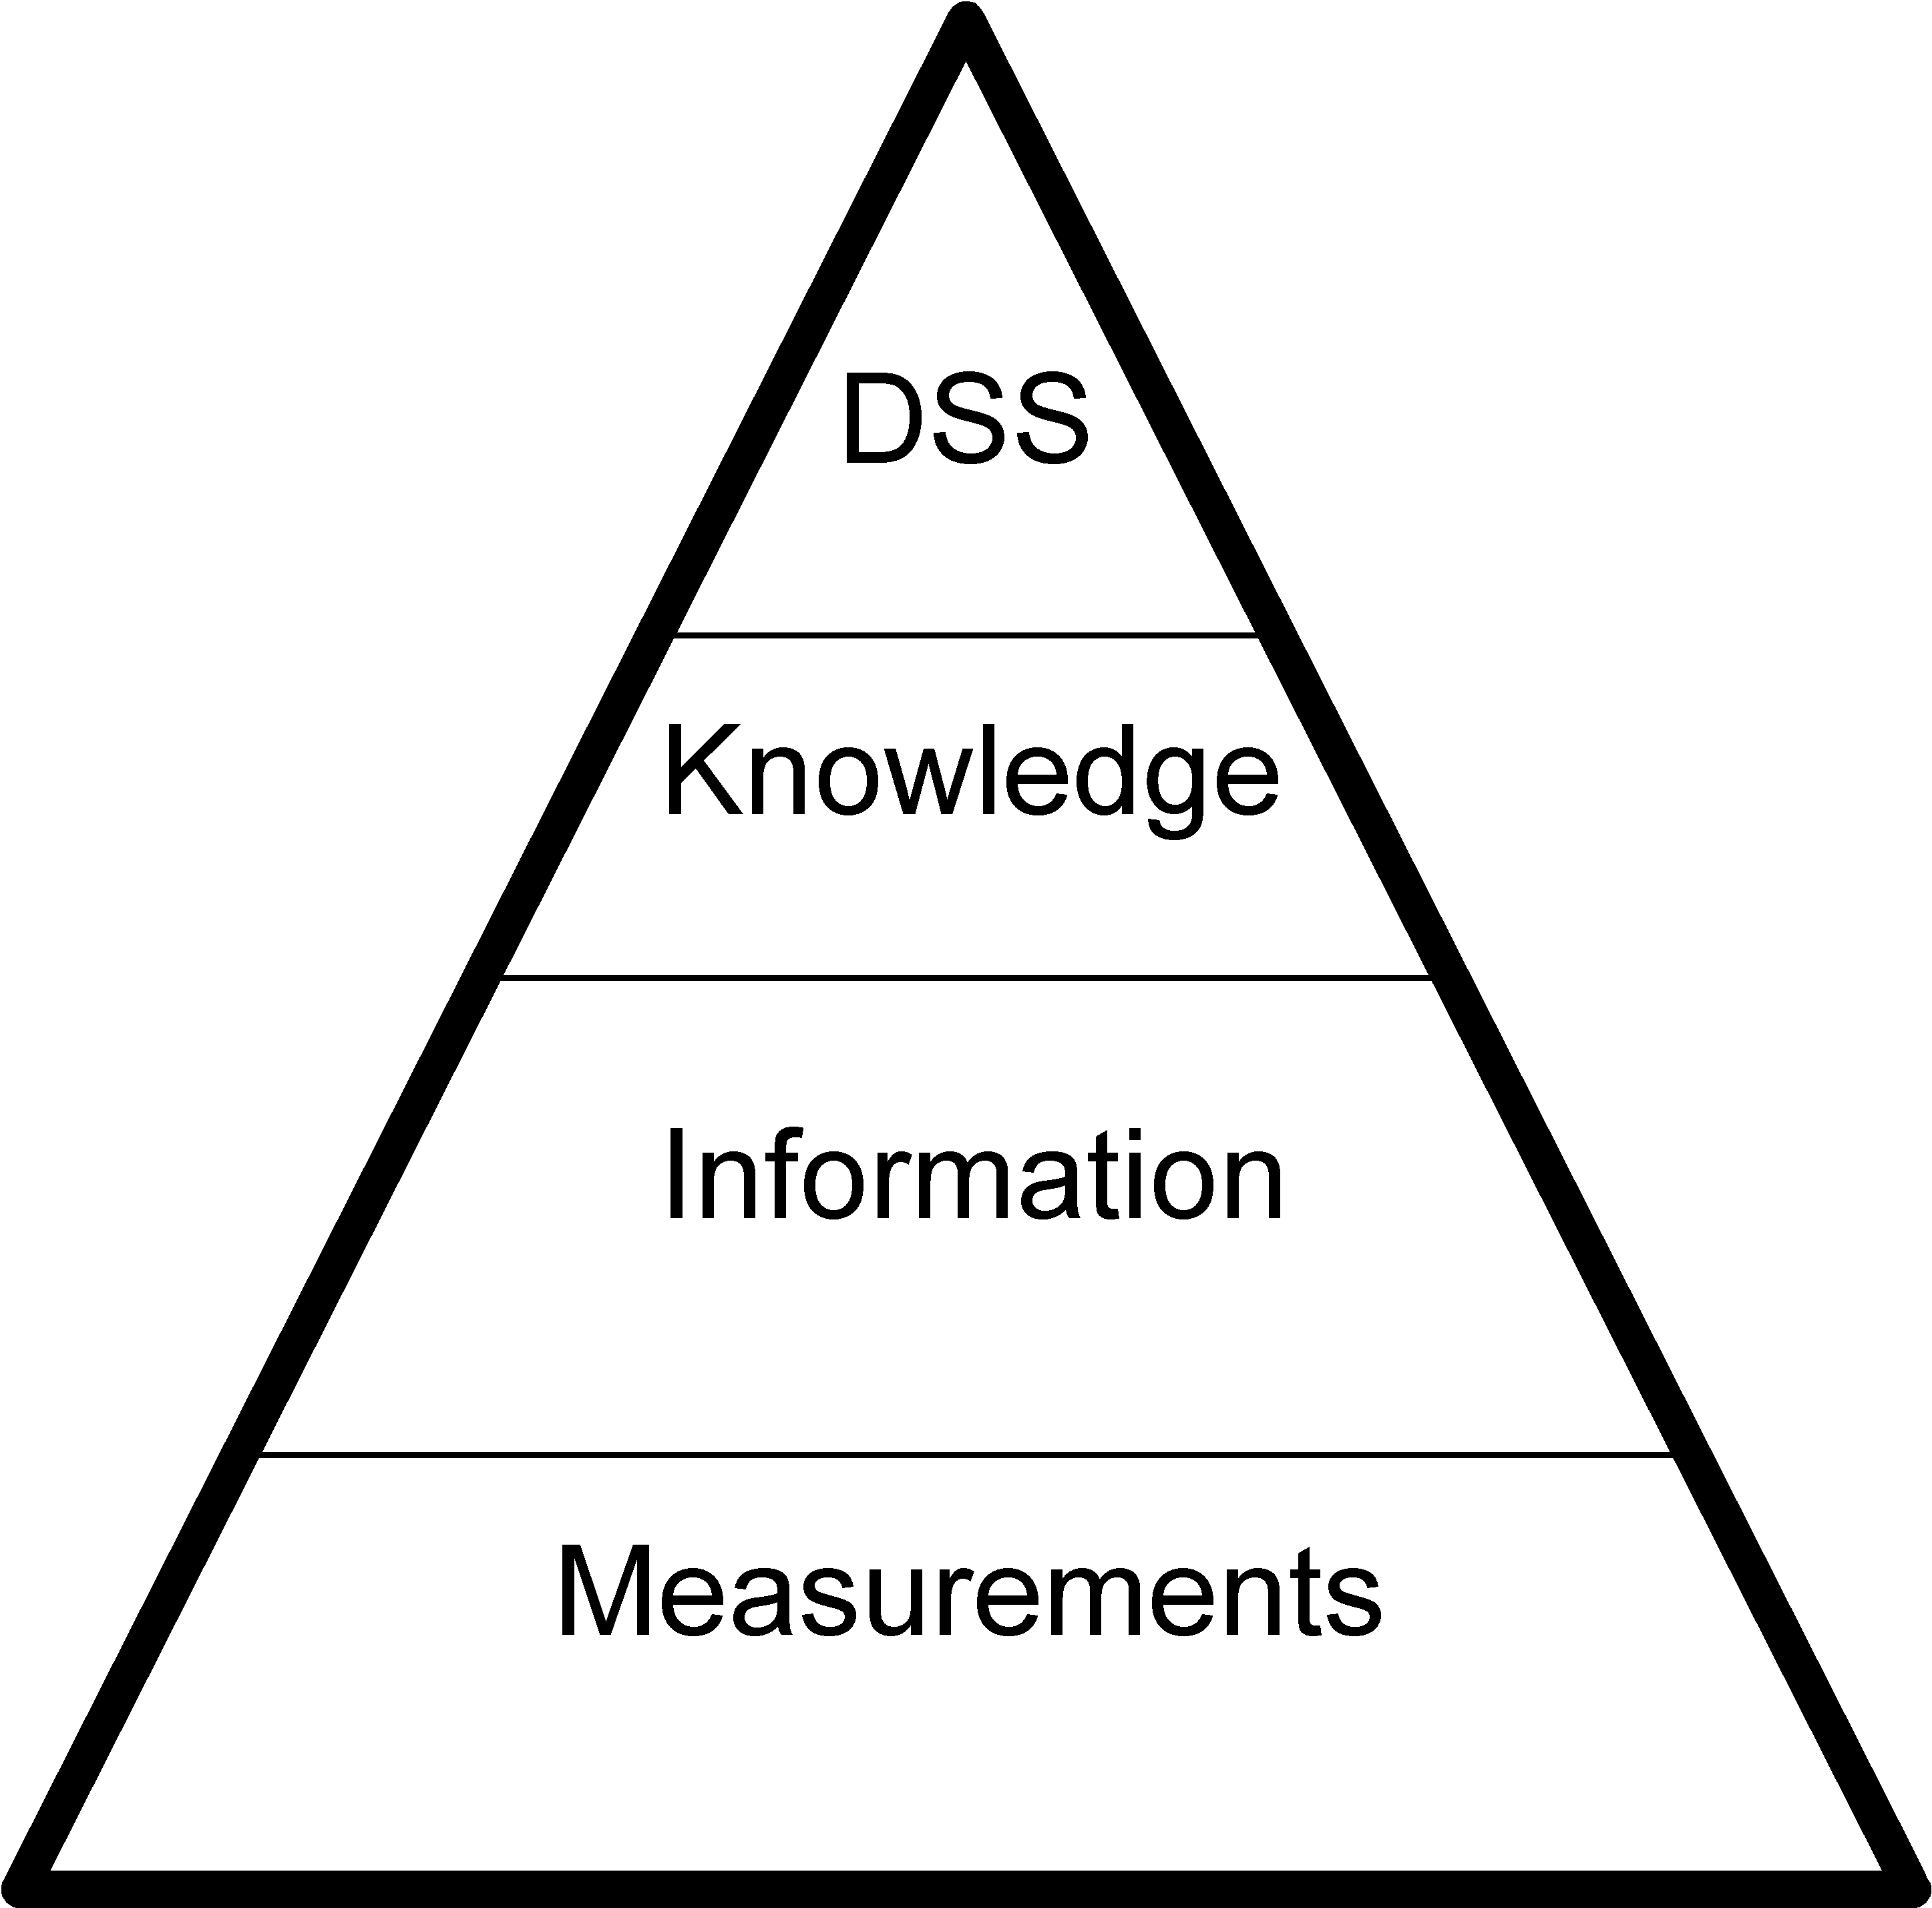
\includegraphics[width=0.3\textwidth,keepaspectratio]{figures/4.Method/pyramid}
	\caption{Overall functional architecture of a smart metering system.}
	\label{fig:41topLevel}
\end{figure}

This work will focus on the first two levels of the smart metering system pyramid. Therefore the energy data must be acquired, processed, transmitted and stored in a centralized database, as represented in figure \ref{fig:41dataFlow}.

\begin{figure}[h!]
	\centering
	
\includegraphics[width=0.8\textwidth,keepaspectratio]{figures/4.Method/data_flow}
	\caption{Data flow of measurement-information layers.}
	\label{fig:41dataFlow}
\end{figure}


For the acquisition part, a non-intrusive self-powered sensor node will be studied. The processing part depends on an accurate knowledge of the catenary and the traction transformer, which depends on train GPS location and power flow conditions. These two parts are further detailed in the methodology and expected contributions of section \ref{sec:42}.

The definition of the processing part will validate if the proposed acquisition architecture has enough support. At this moment a solution with only a current sensor, for the acquisition in each transformer's secondary, is of advanced interest. 

The transmission of the generated information to a centralized storage is further detailed in section \ref{sec:43}. Several models will be considered for accurate simulation of such transmission network. The overall architecture of the system is presented in figure \ref{fig:41architecture}.

\begin{figure}[h!]
	\centering
	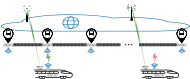
\includegraphics[width=1.0\textwidth,keepaspectratio]{figures/architecture}
	\caption{Architecture of proposed work.}
	\label{fig:41architecture}
\end{figure}







%%%%%%%%%%%%%%%%%%
%%%%%%%%%%%%%%%%%%
%%%%%%%%%%%%%%%%%%
%\newpage
\section{Non-intrusive self-powered sensor node}
\label{sec:42}
\subsection{Purpose}

The purpose of this section is to cover the acquisition and processing parts of the data-flow presented previously. As a starting point, a non-intrusive and self-powered sensor node allows the measurement of AC currents in all transformer secondary windings, as illustrated in figure \ref{fig:4.powerSensing}. This figure is based on the 3400 series train topology of \textit{Comboios de Portugal} (CP) used in urban services.

Based on the field measurements, a data concentrator will receive the current values from each sensor node. This data concentrator generates information based on the estimation of the AC grid voltage and the acquisition of GPS location, as proposed by the European Commission regulation No 1301/2014. For each time-stamp, the active and reactive power is calculated and transmitted together with the geographical position.

In the scope of Shift2Rail, is expected to develop a smart metering system for RTS. Assuming that a non-intrusive measurement system is of extreme interest, this proposal of a non-intrusive and self powered sensor node goes along the goals of Shif2Rail.

On the field of measurement, non-intrusive technical solutions has been used for several years for current measurement, such as hall-effect current sensors, rogowsky probes or current transformers.
For self-powering purposes, some studies on using current transformers for energy harvesting has been proposed in the literature (\cite{ahola2008}, \cite{brunelli2016}, MAIS PAPERS).


\begin{figure}[h!]
	\centering
	\vspace{-1em}
	\includegraphics[width=0.7\textwidth,keepaspectratio]{figures/4.Method/powerSensing}
	\caption{Power architecture of case-study train.}
	\label{fig:4.powerSensing}
\end{figure}



\subsection{Contributions}

\begin{itemize}
	\setlength\itemsep{0em}
	\item New energy metering architecture using a non-intrusive approach.
	
	\item Accurate estimation of injected power into catenary, that is needed for train operation, based on on-board measurements.

\end{itemize}


\subsection{Methodology}

The methodology is divided into two parts. The first part will be related to the processing of the data generated by the sensor nodes and the second part is the definition of the sensor itself.

As a starting point of the methodology, it is expected to work on the \textbf{development of models} similar to the ones presented in figure \ref{fig:4.methodElectrical}. The modeling of such architecture allows the evaluation of the power contribution of a train, at a certain instant, to the power injected to the catenary. This methodology will contribute to \textbf{implementation of processing algorithms} in the train data concentrator that, based on the measurement of AC secondary winding's voltages and currents, will generate the accurate value of the energy injected in the catenary by the traction substation. The expected result will be the comparison between the estimation and the measured injected power in the catenary.

In this second part of the methodology, or the acquisition part, the sensor will be defined and validated. As a first step in the methodology, using Ansys or similar Finit Element Method (FEM) software, the \textbf{current and electric field of one winding will be simulated}. With the results of this simulation, the current and voltage sensors will be evaluated. In a further step, \textbf{real experiments on low voltage test-bench} will test the proposed sensor node.



\begin{figure}[h!]
	\centering
	\includegraphics[width=0.9\textwidth,keepaspectratio]{figures/4.Method/methodElectrical}
	\caption{Models needed for simulation.}
	\label{fig:4.methodElectrical}
\end{figure}



\subsection{Simulation tools and frameworks}

\cite{pilo2000} identifies the need of two tools for the simulation of railway power lines: (1) the simulator for the railway line and (2) an electrical system simulator. Based on that, \cite{almagro2017} uses the simulation tool \textbf{OpenDSS} with the Python integration for the simulation of the railway power lines. A further study on OpenDSS shows enough documentation and recent updates (march 2017) with the possible integration with VBA Excel, MatLAB and Python scripts.

Mathworks suggests also the usage of \textbf{MatLAB and Simulink} for rail electrical systems modeling. 
Similarly, \textbf{Ansys} products are suggested for the simulation of railway power systems as well as \textbf{PSIM}. The three previously presented products are also flexible to work in co-simulation, with the advantage of choosing the best software for the most straightforward application.

\subsection{Preliminary work: evaluation of the non-intrusive voltage sensor}

	A critical issue is identified as the measurement of voltage waveforms using a non-intrusive approach. 
	The work of \cite{brunelli2016} presents a possible non-intrusive voltage measurement for energy meters.
	In this work is referred that, for the authors knowledge, there is no commercially available non-intrusive sensor for voltage measurement in low-voltage wires (230-400 VAC). 
	Despite that, some studies are proposed in the literature for extra/high-voltage monitoring systems based on a capacitive cell.
	
	Based on the solution of \cite{brunelli2016}, a voltage sensor was implemented/tested, as presented in figure \ref{fig:4.voltage_sensor}, with the equivalent circuit in \ref{fig:4.voltage_sensor_eq}. 
	
	
	
	\begin{figure}[h!]
		\centering
		\begin{minipage}{.45\textwidth}
			\centering
			%		\vspace{2.5em}
			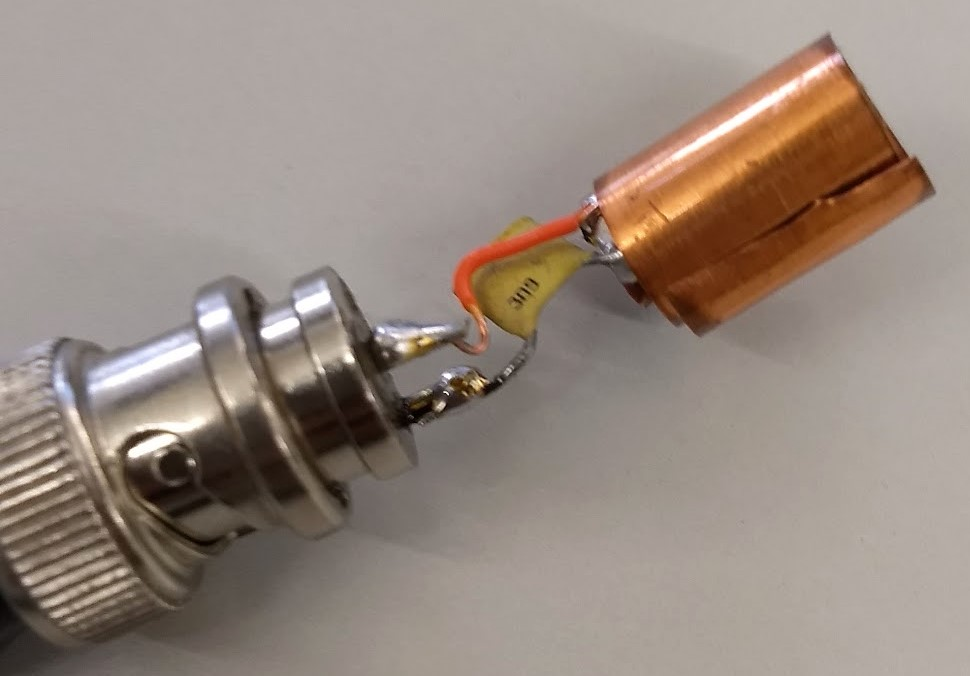
\includegraphics[width=0.8\textwidth,keepaspectratio]{figures/4.Method/voltage_sensor}
			%		\vspace{2em}
			\captionof{figure}{Photo of implemented non-intrusive voltage sensor.}
			\label{fig:4.voltage_sensor}
		\end{minipage}%
		\begin{minipage}{.03\textwidth}  ~\end{minipage}	
		\begin{minipage}{.45\textwidth}
			\centering
			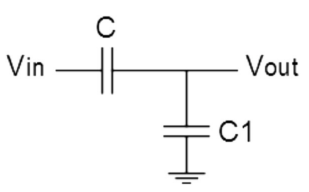
\includegraphics[width=0.9\textwidth,keepaspectratio]{figures/4.Method/voltage_sensor_eq}
			%		\vspace{2em}
			\captionof{figure}{Equivalent circuit of non-intrusive voltage sensor.}
			\label{fig:4.voltage_sensor_eq}
		\end{minipage}
	\end{figure}

	
	To evaluate this sensor, two tests was performed: one with normal conditions of the grid, and other near a Voltage Source Converter (VSC), respectively in figure \ref{fig:4.scope_0} and \ref{fig:4.scope_2}. 
	The VSC is connected to the grid with a low-frequency transformer, which results in a line-to-line voltage of 200V (RMS) in the VSC, \cite{martins2016}.
	
		\begin{figure}[h!]
		\centering
		\begin{minipage}{.45\textwidth}
			\centering
			%		\vspace{2.5em}
			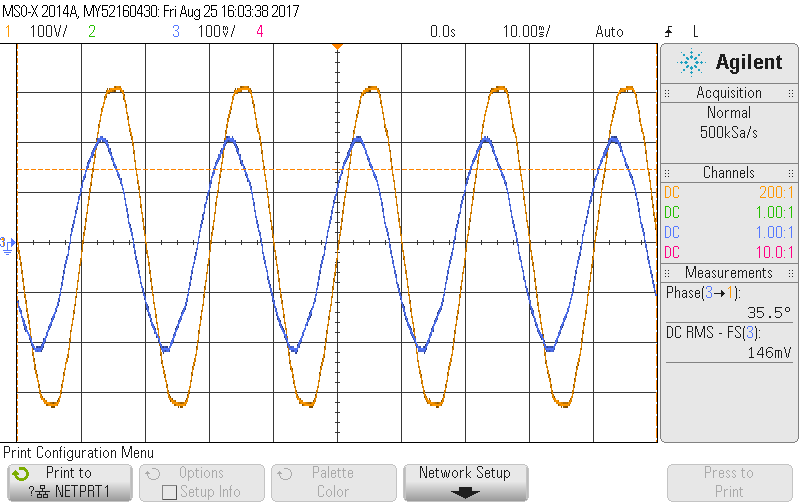
\includegraphics[width=\textwidth,keepaspectratio]{figures/4.Method/scope_0}
			%		\vspace{2em}
			\captionof{figure}{Waveforms of acquired and sensed voltages in normal conditions: (orange) AC main voltage and (blue) voltage in sensor.}
			\label{fig:4.scope_0}
		\end{minipage}%
		\begin{minipage}{.03\textwidth}  ~\end{minipage}	
		\begin{minipage}{.45\textwidth}
			\centering
			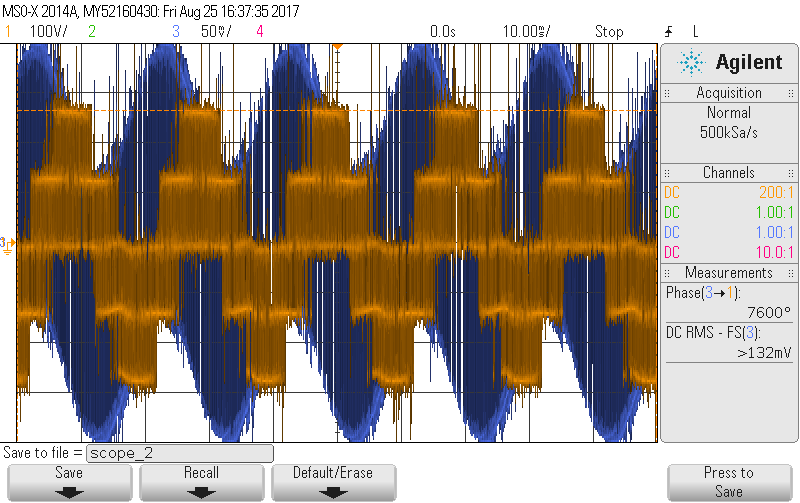
\includegraphics[width=\textwidth,keepaspectratio]{figures/4.Method/scope_2}
			%		\vspace{2em}
			\captionof{figure}{Waveforms of acquired and sensed voltages in inverter: (orange) AC main voltage and (blue) voltage in sensor.}
			\label{fig:4.scope_2}
		\end{minipage}
	\end{figure}

	The purpose of this preliminary work is to evaluate if this solution presented in the state of the art is feasible to be implemented in an environment with huge amount of noise. At first evaluation the answer is negative, due to the need of extra work to estimate the voltage using the blue waveform of figure \ref{fig:4.scope_2}.
	If it is possible to extract the voltage waveform, this can be considered as a contribution to the field of voltage measurement in noisy environments, and in particular, in the railway environment.
	Therefore and as previously presented in the second part of the methodology, the future work will start with the simulation of the electric field in a wire subjected to a VSC and the implementation of a solution that extracts the "real" voltage from the signal of the voltage sensor.
	
	
%%%%%%%%%%%%%%%
%%%%%%%%%%%%%%%
%%%%%%%%%%%%%%%

\section{RTS wireless network}
\label{sec:43}

\subsection{Purpose}

The main purpose of the RTS wireless network is to transmit energy measurements and information generated by the nodes to a centralized storage server. 

As a lower level and as previously presented, each train has current sensors as nodes and a data concentrator. Between nodes and data concentrator, AC voltage and current measurements must be exchanged.
At this level, the relevant issue will be the energy consumption of nodes.

Between train data concentrator and ground-level, the train movement should be considered to better comply with the purpose of transmission the information generated at trains to the centralized storage server. 

Further modeling and simulation of a WSN for energy measurement of RTS rolling stock will be made.

\subsection{Contribution}
%An energy measurement system in rolling stock does not require a broadband real-time/continuous communication (such as LTE), being possible to collect and store data in train data concentrator and, while the train is waiting at station for passenger exchange (which lasts for less than one minute), the data is transferred between train and station AP (and then to a remote server). Therefore, the contribution will be the cost reduction of information transmission of energy sensor network data

\begin{itemize}
	\setlength\itemsep{0em}
	
	\item As a starting point, one contribution will be the availability of measured data from trains where currently no energy measurement is performed.
	
	\item A second contribution will be the data-rate increasing of energy measurements, which will result on direct increase on the quality of information of energy.
	
	\item A further contribution can be the avoidance of broadband real-time/continuous communication (such as LTE), being possible to collect and store data in train data concentrator and, while the train is waiting at stations, the data is transferred between train and station AP (and then to a remote server). A possible contribution will be the cost reduction of information transmission of energy sensor network data.
\end{itemize}

\subsection{Methodology}

The methodology for this part will include the \textbf{modeling and simulation} of network blocks similar to the ones presented in figure \ref{fig:4.methodWireless}. An accurate modeling and simulation will define the more appropriate network technologies to implement in this RTS network. 
The simulation will be performed in a NS-3 simulator or similar.
The \textbf{results} of such simulation will define the max data-rate of the sensor nodes as well as the energy consumption required for the information transmission.

\begin{figure}[h!]
	\centering
	\includegraphics[width=0.9\textwidth,keepaspectratio]{figures/4.Method/methodWireless}
	\caption{Models needed for simulation.}
	\label{fig:4.methodWireless}
\end{figure}

\subsection{Simulation tools and frameworks}

Several simulators/emulators were presented in the literature review chapter. From those, special attention is given to the NS-3 simulator and the MatLAB/Simulink tool.  
%<<necessário avaliar melhor os restantes candidatos>>

\subsection{Preliminary work: implementation of a point-to-point communication between a moving train and a station}



\section{Work plan}
\label{sec:44}

To be defined.

Secondary tasks of the work plan are the deliverables for the iRail programme and for the FCT institution, which occurs at end of academic year. 




%\chapter{Preliminary Work}
%\input{chapters/4.Preliminary}



\bibliographystyle{chicago}
%chicago}

%nota: não ter espaços entre ficheiros
\bibliography{bib/shift2rail,bib/references,bib/31.SmartM,bib/32.WirelessN,bib/33.EnergyS,bib/34.PowerS,bib/35.DSS,bib/36.OutlierD}
%\bibliography{outliers}
%\PrintBib{outliers, }


%\bibliographystyle{plainnat}
%\bibliography{references}

%\chapter*{Attachment 1 --- \large{Overview of communication systems for Smart Grids}}
%\includepdf[pages=-, scale=0.9, offset=-10 0, pagecommand={\thispagestyle{plain}}]  {chapters/communication}


\end{document}